% Options for packages loaded elsewhere
\PassOptionsToPackage{unicode}{hyperref}
\PassOptionsToPackage{hyphens}{url}
\PassOptionsToPackage{dvipsnames,svgnames,x11names}{xcolor}
%
\documentclass[
  letterpaper,
  DIV=11,
  numbers=noendperiod]{scrartcl}

\usepackage{amsmath,amssymb}
\usepackage{iftex}
\ifPDFTeX
  \usepackage[T1]{fontenc}
  \usepackage[utf8]{inputenc}
  \usepackage{textcomp} % provide euro and other symbols
\else % if luatex or xetex
  \usepackage{unicode-math}
  \defaultfontfeatures{Scale=MatchLowercase}
  \defaultfontfeatures[\rmfamily]{Ligatures=TeX,Scale=1}
\fi
\usepackage{lmodern}
\ifPDFTeX\else  
    % xetex/luatex font selection
\fi
% Use upquote if available, for straight quotes in verbatim environments
\IfFileExists{upquote.sty}{\usepackage{upquote}}{}
\IfFileExists{microtype.sty}{% use microtype if available
  \usepackage[]{microtype}
  \UseMicrotypeSet[protrusion]{basicmath} % disable protrusion for tt fonts
}{}
\makeatletter
\@ifundefined{KOMAClassName}{% if non-KOMA class
  \IfFileExists{parskip.sty}{%
    \usepackage{parskip}
  }{% else
    \setlength{\parindent}{0pt}
    \setlength{\parskip}{6pt plus 2pt minus 1pt}}
}{% if KOMA class
  \KOMAoptions{parskip=half}}
\makeatother
\usepackage{xcolor}
\setlength{\emergencystretch}{3em} % prevent overfull lines
\setcounter{secnumdepth}{-\maxdimen} % remove section numbering
% Make \paragraph and \subparagraph free-standing
\makeatletter
\ifx\paragraph\undefined\else
  \let\oldparagraph\paragraph
  \renewcommand{\paragraph}{
    \@ifstar
      \xxxParagraphStar
      \xxxParagraphNoStar
  }
  \newcommand{\xxxParagraphStar}[1]{\oldparagraph*{#1}\mbox{}}
  \newcommand{\xxxParagraphNoStar}[1]{\oldparagraph{#1}\mbox{}}
\fi
\ifx\subparagraph\undefined\else
  \let\oldsubparagraph\subparagraph
  \renewcommand{\subparagraph}{
    \@ifstar
      \xxxSubParagraphStar
      \xxxSubParagraphNoStar
  }
  \newcommand{\xxxSubParagraphStar}[1]{\oldsubparagraph*{#1}\mbox{}}
  \newcommand{\xxxSubParagraphNoStar}[1]{\oldsubparagraph{#1}\mbox{}}
\fi
\makeatother


\providecommand{\tightlist}{%
  \setlength{\itemsep}{0pt}\setlength{\parskip}{0pt}}\usepackage{longtable,booktabs,array}
\usepackage{calc} % for calculating minipage widths
% Correct order of tables after \paragraph or \subparagraph
\usepackage{etoolbox}
\makeatletter
\patchcmd\longtable{\par}{\if@noskipsec\mbox{}\fi\par}{}{}
\makeatother
% Allow footnotes in longtable head/foot
\IfFileExists{footnotehyper.sty}{\usepackage{footnotehyper}}{\usepackage{footnote}}
\makesavenoteenv{longtable}
\usepackage{graphicx}
\makeatletter
\def\maxwidth{\ifdim\Gin@nat@width>\linewidth\linewidth\else\Gin@nat@width\fi}
\def\maxheight{\ifdim\Gin@nat@height>\textheight\textheight\else\Gin@nat@height\fi}
\makeatother
% Scale images if necessary, so that they will not overflow the page
% margins by default, and it is still possible to overwrite the defaults
% using explicit options in \includegraphics[width, height, ...]{}
\setkeys{Gin}{width=\maxwidth,height=\maxheight,keepaspectratio}
% Set default figure placement to htbp
\makeatletter
\def\fps@figure{htbp}
\makeatother

\KOMAoption{captions}{tableheading}
\makeatletter
\@ifpackageloaded{caption}{}{\usepackage{caption}}
\AtBeginDocument{%
\ifdefined\contentsname
  \renewcommand*\contentsname{Table of contents}
\else
  \newcommand\contentsname{Table of contents}
\fi
\ifdefined\listfigurename
  \renewcommand*\listfigurename{List of Figures}
\else
  \newcommand\listfigurename{List of Figures}
\fi
\ifdefined\listtablename
  \renewcommand*\listtablename{List of Tables}
\else
  \newcommand\listtablename{List of Tables}
\fi
\ifdefined\figurename
  \renewcommand*\figurename{Figure}
\else
  \newcommand\figurename{Figure}
\fi
\ifdefined\tablename
  \renewcommand*\tablename{Table}
\else
  \newcommand\tablename{Table}
\fi
}
\@ifpackageloaded{float}{}{\usepackage{float}}
\floatstyle{ruled}
\@ifundefined{c@chapter}{\newfloat{codelisting}{h}{lop}}{\newfloat{codelisting}{h}{lop}[chapter]}
\floatname{codelisting}{Listing}
\newcommand*\listoflistings{\listof{codelisting}{List of Listings}}
\makeatother
\makeatletter
\makeatother
\makeatletter
\@ifpackageloaded{caption}{}{\usepackage{caption}}
\@ifpackageloaded{subcaption}{}{\usepackage{subcaption}}
\makeatother

\ifLuaTeX
  \usepackage{selnolig}  % disable illegal ligatures
\fi
\usepackage{bookmark}

\IfFileExists{xurl.sty}{\usepackage{xurl}}{} % add URL line breaks if available
\urlstyle{same} % disable monospaced font for URLs
\hypersetup{
  pdftitle={A Compact Study on Public Readiness for the Smart Grid in India},
  colorlinks=true,
  linkcolor={blue},
  filecolor={Maroon},
  citecolor={Blue},
  urlcolor={Blue},
  pdfcreator={LaTeX via pandoc}}


\title{A Compact Study on Public Readiness for the Smart Grid in India}
\author{Siju K S \and Abhijith M S}
\date{}

\begin{document}
\maketitle
\begin{abstract}
This study investigates generational differences in energy consumption
patterns and attitudes towards smart grid technologies among Generation
Z and Millennials. Utilizing a cross-sectional survey design, data was
collected from 498 respondents through stratified random sampling. The
analysis reveals a strong preference for online bill payment methods,
indicating a readiness for digital solutions like smart meters. However,
a significant portion of respondents still rely on physical payment
methods, highlighting the need for targeted educational initiatives. The
study emphasizes the importance of adaptive communication strategies to
the specific needs of each generation. For Generation Z, educational
outreach focusing on the practical benefits of smart meters is
effective, while Millennials respond better to data-centric
communication addressing privacy concerns. These findings provide
valuable insights for policymakers and stakeholders to develop targeted
initiatives promoting energy efficiency and sustainability. Future
research should expand the demographic scope to capture a broader range
of perspectives and provide deeper insights into technology adoption
factors.
\end{abstract}


\subsection{Introduction}\label{introduction}

The global energy landscape is undergoing a paradigm shift.
Environmental concerns and the burgeoning demand for sustainable
solutions are driving the evolution of intelligent and efficient power
grids, with smart meters playing a pivotal role. These advanced devices
capture real-time energy consumption data, enabling two-way
communication between utilities and consumers. However, for a seamless
integration of smart meters, garnering public acceptance and fostering a
culture of informed energy use is paramount. This study delves into the
feasibility of implementing smart meters in a specific region through a
comprehensive survey analysis. We employ a multi-pronged approach,
focusing on three key areas: public perception of smart meters,
attitudes towards energy-saving technologies, and interest in emerging
advancements like rooftop solar and electric vehicles. Additionally, we
explore how demographic factors influence these perspectives. To gain a
deeper understanding of consumer behavior, we will develop a
segmentation strategy. This approach involves categorizing smart meter
users into distinct groups based on their viewpoints towards energy
consumption. By identifying these segments, we can knitdown
communication strategies and targeted interventions to resonate more
effectively with each group. For instance, one segment might comprise
environmentally conscious consumers who readily adopt smart meters and
energy-saving technologies. Another segment might be more
cost-conscious, requiring clear demonstrations of cost savings
associated with smart meters.

\subsubsection{The Global Rise of Smart
Technologies}\label{the-global-rise-of-smart-technologies}

The groundwork for smart grid adoption is already being laid. As of late
2023, over 1.06 billion smart meters (electricity, water, and gas) have
been installed worldwide, signifying a pivotal step towards modernizing
utility infrastructure {[}1{]}. Notably, North America leads the pack
with a staggering 77\% penetration rate for smart electricity meters,
highlighting the growing maturity of this market {[}2{]}.

\subsubsection{Significance of the
study}\label{significance-of-the-study}

By investigating these areas and employing segmentation techniques, this
study will provide valuable insights into public readiness for smart
meters and the broader smart grid ecosystem. This information will
empower stakeholders to develop targeted initiatives and craft
communication strategies that resonate with specific consumer segments.
Ultimately, this comprehensive approach will pave the way for a smoother
transition towards a more sustainable and efficient energy future.
Understanding the perceptions and behaviors of different demographic
groups towards energy consumption and technology adoption is crucial for
designing effective policies and interventions. This study aims to
bridge the knowledge gap by providing insights into the generational
differences in energy consumption patterns, technology adoption, and
perceptions of various energy-saving initiatives. The findings of this
study can inform targeted communication strategies and policy decisions
to promote energy efficiency and sustainability.

\subsubsection{Objectives of the Study}\label{objectives-of-the-study}

The primary objectives of this study are to assess generational
differences in energy consumption and technology adoption, examine the
impact of home ownership and size on energy consumption, analyze
perceptions of data privacy and load control programs, and evaluate the
statistical reliability and normality of constructs.

Firstly, the study aims to \emph{evaluate how Generation Z and
Millennials differ in their energy consumption patterns, willingness to
adopt smart grid technologies, and perceptions of various energy-saving
initiatives such as smart meters, rooftop PV systems, electric vehicles
(EVs), and vehicle-to-grid (V2G) technology}. Understanding these
differences is crucial for tailoring communication strategies and
interventions to effectively engage each generation, thereby enhancing
the adoption of energy-efficient technologies.

Secondly, the study \emph{investigates the relationship between home
ownership status, home size, and energy consumption profiles, and how
these factors influence the adoption of energy-efficient technologies}.
Home ownership and size are significant determinants of energy
consumption. Analyzing these factors can provide insights into the
specific needs and challenges faced by different household types,
enabling more targeted and effective energy-saving measures.

Lastly, the study \emph{seeks to understand respondents' comfort levels
with sharing energy consumption data and participating in load control
programs, and to identify any generational differences in these
perceptions}. Data privacy concerns and willingness to participate in
load control programs are critical factors influencing the adoption of
smart grid technologies. Addressing these concerns through informed
communication can enhance public acceptance and participation.

In summary, this study's objectives are designed to provide a
comprehensive understanding of the factors influencing energy
consumption and technology adoption across different generations. The
insights gained can inform targeted strategies to promote energy
efficiency and sustainability, addressing the unique needs and concerns
of various demographic groups.

\subsection{Methodology}\label{methodology}

A systematic research methodology is crucial for ensuring the
reliability and validity of findings in studies examining energy
consumption and technology adoption. This study employs a rigorous
cross-sectional survey design to gather comprehensive data on the
behaviors and attitudes of Generation Z and Millennials. By utilizing
stratified random sampling, the study ensures a representative sample
that captures diverse demographic variables. The use of robust
statistical analyses, including descriptive statistics, reliability
tests, normality tests, cross-tabulation, and ANOVA, allows for a
thorough examination of the data and identification of significant
patterns and differences. Ethical considerations, such as informed
consent and data confidentiality, are meticulously adhered to, ensuring
the integrity of the research process. This systematic approach not only
enhances the credibility of the study's findings but also provides
valuable insights that can inform targeted strategies for promoting
energy efficiency and sustainability.

\subsubsection{Study Design}\label{study-design}

This study employs a cross-sectional survey design to collect data on
energy consumption patterns, technology adoption, and perceptions of
various energy-saving initiatives among Generation Z and Millennials.
The survey includes a combination of quantitative and qualitative
questions to capture a comprehensive view of respondents' behaviors and
attitudes.

\subsubsection{Sample Selection}\label{sample-selection}

The sample consists of 498 respondents, divided into two generational
cohorts: Generation Z (273 respondents) and Millennials (225
respondents). Participants were selected using stratified random
sampling to ensure representation across different demographic variables
such as gender, home ownership status, and geographic location.

\subsubsection{Data Collection}\label{data-collection}

Data was collected through an online survey distributed via email and
social media platforms. The survey included sections on demographic
information, energy consumption patterns, perceptions of smart grid
technologies, willingness to share energy consumption data, and
attitudes towards load control programs and vehicle-to-grid (V2G)
technology. Respondents were asked to rate their perceptions using
Likert-scale items.

\subsubsection{Variables and Measures}\label{variables-and-measures}

\begin{itemize}
\tightlist
\item
  \textbf{Demographic Variables}: Age, gender, home ownership status,
  and geographic location.
\item
  \textbf{Energy Consumption Patterns}: Self-reported energy usage and
  willingness to optimize energy consumption.
\item
  \textbf{Technology Adoption}: Perceptions of smart grid technologies,
  rooftop PV systems, electric vehicles (EVs), and V2G technology.
\item
  \textbf{Data Privacy and Load Control}: Comfort levels with sharing
  energy consumption data and participating in load control programs.
\end{itemize}

\subsubsection{Statistical Analysis}\label{statistical-analysis}

Data analysis was conducted using SPSS software. The following
statistical tests and procedures were employed:

\begin{enumerate}
\def\labelenumi{\arabic{enumi}.}
\tightlist
\item
  \textbf{Descriptive Statistics}: To summarize the demographic
  characteristics of the sample and the distribution of responses for
  each variable.
\item
  \textbf{Reliability Analysis}: Cronbach's alpha was used to assess the
  internal consistency of the constructs.
\item
  \textbf{Normality Tests}: Kolmogorov-Smirnov and Shapiro-Wilk tests
  were conducted to check the normality of the constructs.
\item
  \textbf{Cross-tabulation}: To examine the relationship between
  categorical variables such as home ownership status and energy
  consumption profiles.
\item
  \textbf{ANOVA (Analysis of Variance)}: To assess significant
  differences in perceptions and behaviors between Generation Z and
  Millennials.
\item
  \textbf{Box-Cox Transformation}: Applied to normalize the data where
  necessary.
\end{enumerate}

\subsubsection{Ethical Considerations}\label{ethical-considerations}

The study was conducted in accordance with ethical guidelines for
research involving human participants. Informed consent was obtained
from all respondents, and data confidentiality was maintained throughout
the study. Participants were assured that their responses would be
anonymized and used solely for research purposes.

\subsubsection{Limitations}\label{limitations}

The study acknowledges potential limitations, including self-report bias
and the representativeness of the sample. Future research could expand
the sample size and include additional demographic variables to enhance
the generalizability of the findings.

In summary, this methodology outlines a rigorous approach to
investigating generational differences in energy consumption and
technology adoption, providing valuable insights to inform targeted
strategies for promoting energy efficiency and sustainability.

\subsection{Results and Discussions}\label{results-and-discussions}

\subsubsection{Baseline Analysis}\label{baseline-analysis}

The baseline analysis provides an overview of the demographic
characteristics of the study sample, setting the stage for a deeper
understanding of the factors influencing energy consumption and
technology adoption. By examining variables such as gender, age, home
ownership status, and geographic distribution, this section establishes
a foundational context for interpreting the subsequent findings. The
demographic breakdown helps ensure that the sample is representative of
the broader population, thereby enhancing the generalizability of the
study's conclusions. This initial analysis is crucial for identifying
any inherent biases or patterns that may influence the overall results
and for validating the robustness of the data collected.

The gender-wise percentage analysis is shown in Table~\ref{tbl-gender}.

\begin{longtable}[]{@{}llll@{}}
\caption{Gender-wise percentage analysis of the data
collected}\label{tbl-gender}\tabularnewline
\toprule\noalign{}
Frequency & Percent & Valid Percent & Cumulative Percent \\
\midrule\noalign{}
\endfirsthead
\toprule\noalign{}
Frequency & Percent & Valid Percent & Cumulative Percent \\
\midrule\noalign{}
\endhead
\bottomrule\noalign{}
\endlastfoot
Female & 119 & 23.9 & 23.9 \\
Male & 379 & 76.1 & 100.0 \\
Total & 498 & 100.0 & 100.0 \\
\end{longtable}

Table Table~\ref{tbl-gender} presents the gender-wise classification of
data collected through a multi-stage random sampling process across
various states in India. The sample consists of 498 individuals, with
23.9\% identified as female and 76.1\% as male. The cumulative
percentage indicates that the entire sample has been accounted for, with
males comprising the majority of the respondents.

\subsubsection{Types of Respondents}\label{types-of-respondents}

The percentage of respondent over Generation type is shown in
Table~\ref{tbl-generation}.

\begin{longtable}[]{@{}llll@{}}
\caption{Generation-wise percentage analysis of the data
collected}\label{tbl-generation}\tabularnewline
\toprule\noalign{}
Frequency & Percent & Valid Percent & Cumulative Percent \\
\midrule\noalign{}
\endfirsthead
\toprule\noalign{}
Frequency & Percent & Valid Percent & Cumulative Percent \\
\midrule\noalign{}
\endhead
\bottomrule\noalign{}
\endlastfoot
Generation Z & 273 & 54.8 & 54.8 \\
Millennials & 225 & 45.2 & 100.0 \\
Total & 498 & 100.0 & 100.0 \\
\end{longtable}

Table~\ref{tbl-generation} presents the generation-wise classification
of data collected through a multi-stage random sampling process across
various states in India. The sample consists of 498 individuals, with
54.8\% identified as Generation Z and 45.2\% as Millennials. The
cumulative percentage indicates that the entire sample has been
accounted for, with Generation Z comprising the majority of the
respondents.

The survey contains Generation Z (54.8\%) and Millennials (45.2\%).
According to a Pew Research Center study
\url{https://www.pewresearch.org/social-trends/2020/05/14/on-the-cusp-of-adulthood-and-facing-an-uncertain-future-what-we-know-about-gen-z-so-far-2/},
both generations are known for their tech-savviness and adoption of new
technologies. This suggests that the survey results may be particularly
relevant for understanding public perception of smart grid technologies,
as both generations are likely to be comfortable with and interested in
new devices and applications. However, it's important to consider some
behavioral nuances between these generations:

\begin{itemize}
\item
  Millennials: Having grown up with the internet and personal computers,
  Millennials may be more familiar with smart home devices and be
  comfortable managing them through apps. They might prioritize the
  financial benefits of smart meters, like potential cost savings
  through real-time energy monitoring.
\item
  Generation Z: This generation has grown up surrounded by even more
  advanced technologies like smartphones and social media. They may be
  more concerned about data privacy and security when it comes to smart
  meters. Additionally, Gen Z is known for being particularly
  environmentally conscious, so they might be receptive to smart meters
  if they understand the environmental benefits of reduced energy
  consumption.
\end{itemize}

By understanding these potential differences in attitudes, policymakers
and utility companies can tailor their communication strategies to
resonate with each generation. For example, highlighting cost savings
might be more effective for Millennials, while emphasizing environmental
benefits could be a stronger motivator for Gen Z.

\subsubsection{State-wise Analysis}\label{state-wise-analysis}

A state-wise percentage is shown in the following Table.

\begin{longtable}[]{@{}
  >{\raggedright\arraybackslash}p{(\columnwidth - 8\tabcolsep) * \real{0.2857}}
  >{\raggedright\arraybackslash}p{(\columnwidth - 8\tabcolsep) * \real{0.1429}}
  >{\raggedright\arraybackslash}p{(\columnwidth - 8\tabcolsep) * \real{0.1169}}
  >{\raggedright\arraybackslash}p{(\columnwidth - 8\tabcolsep) * \real{0.1948}}
  >{\raggedright\arraybackslash}p{(\columnwidth - 8\tabcolsep) * \real{0.2597}}@{}}
\caption{State-wise percentage analysis of the data
collected}\label{tbl-state}\tabularnewline
\toprule\noalign{}
\begin{minipage}[b]{\linewidth}\raggedright
State
\end{minipage} & \begin{minipage}[b]{\linewidth}\raggedright
Frequency
\end{minipage} & \begin{minipage}[b]{\linewidth}\raggedright
Percent
\end{minipage} & \begin{minipage}[b]{\linewidth}\raggedright
Valid Percent
\end{minipage} & \begin{minipage}[b]{\linewidth}\raggedright
Cumulative Percent
\end{minipage} \\
\midrule\noalign{}
\endfirsthead
\toprule\noalign{}
\begin{minipage}[b]{\linewidth}\raggedright
State
\end{minipage} & \begin{minipage}[b]{\linewidth}\raggedright
Frequency
\end{minipage} & \begin{minipage}[b]{\linewidth}\raggedright
Percent
\end{minipage} & \begin{minipage}[b]{\linewidth}\raggedright
Valid Percent
\end{minipage} & \begin{minipage}[b]{\linewidth}\raggedright
Cumulative Percent
\end{minipage} \\
\midrule\noalign{}
\endhead
\bottomrule\noalign{}
\endlastfoot
Andhra Pradesh & 12 & 2.4 & 2.4 & 2.4 \\
Assam & 3 & 0.6 & 0.6 & 3.0 \\
Bihar & 13 & 2.6 & 2.6 & 5.6 \\
Delhi & 9 & 1.8 & 1.8 & 7.4 \\
Gujarat & 1 & 0.2 & 0.2 & 7.6 \\
Haryana & 4 & 0.8 & 0.8 & 8.4 \\
Jammu and Kashmir & 6 & 1.2 & 1.2 & 9.6 \\
Jharkhand & 3 & 0.6 & 0.6 & 10.2 \\
Karnataka & 8 & 1.6 & 1.6 & 11.8 \\
Kerala & 220 & 44.2 & 44.2 & 56.0 \\
Madhya Pradesh & 5 & 1.0 & 1.0 & 57.0 \\
Maharashtra & 2 & 0.4 & 0.4 & 57.4 \\
Meghalaya & 2 & 0.4 & 0.4 & 57.8 \\
Punjab & 1 & 0.2 & 0.2 & 58.0 \\
Rajastan & 1 & 0.2 & 0.2 & 58.2 \\
Rajasthan & 12 & 2.4 & 2.4 & 60.6 \\
Tamil Nadu & 13 & 2.6 & 2.6 & 63.3 \\
Telangana & 6 & 1.2 & 1.2 & 64.5 \\
Uttar Pradesh & 79 & 15.9 & 15.9 & 80.3 \\
Uttarakhand & 96 & 19.3 & 19.3 & 99.6 \\
West Bengal & 2 & 0.4 & 0.4 & 100.0 \\
Total & 498 & 100.0 & 100.0 & 100.0 \\
\end{longtable}

Table~\ref{tbl-state} presents the state-wise classification of data
collected through a multi-stage random sampling process across various
states in India. The sample consists of 498 individuals, with the
highest representation from Kerala (44.2\%), followed by Uttar Pradesh
(15.9\%) and Uttarakhand (19.3\%). The cumulative percentage indicates
that the entire sample has been accounted for, with Kerala comprising
the majority of the respondents.

It is important to note the sample imbalance across states, with a
significant overrepresentation from Kerala. This imbalance may impact
the study's findings, as the views and behaviors of respondents from
Kerala could disproportionately influence the overall results.
Consequently, the conclusions drawn may not fully represent the
diversity of opinions and behaviors across all states in India. Future
studies should aim for a more balanced sample distribution to ensure
more generalizable and representative findings.

\subsubsection{Educational Background of Survey Respondents: Tailored
for Highly Educated
Spectrum}\label{educational-background-of-survey-respondents-tailored-for-highly-educated-spectrum}

The percentage of respondents over educational qualification is shown in
Table~\ref{tbl-education}.

\begin{longtable}[]{@{}
  >{\raggedright\arraybackslash}p{(\columnwidth - 8\tabcolsep) * \real{0.2857}}
  >{\raggedright\arraybackslash}p{(\columnwidth - 8\tabcolsep) * \real{0.1429}}
  >{\raggedright\arraybackslash}p{(\columnwidth - 8\tabcolsep) * \real{0.1169}}
  >{\raggedright\arraybackslash}p{(\columnwidth - 8\tabcolsep) * \real{0.1948}}
  >{\raggedright\arraybackslash}p{(\columnwidth - 8\tabcolsep) * \real{0.2597}}@{}}
\caption{Educational qualification percentage analysis of the data
collected}\label{tbl-education}\tabularnewline
\toprule\noalign{}
\begin{minipage}[b]{\linewidth}\raggedright
Education
\end{minipage} & \begin{minipage}[b]{\linewidth}\raggedright
Frequency
\end{minipage} & \begin{minipage}[b]{\linewidth}\raggedright
Percent
\end{minipage} & \begin{minipage}[b]{\linewidth}\raggedright
Valid Percent
\end{minipage} & \begin{minipage}[b]{\linewidth}\raggedright
Cumulative Percent
\end{minipage} \\
\midrule\noalign{}
\endfirsthead
\toprule\noalign{}
\begin{minipage}[b]{\linewidth}\raggedright
Education
\end{minipage} & \begin{minipage}[b]{\linewidth}\raggedright
Frequency
\end{minipage} & \begin{minipage}[b]{\linewidth}\raggedright
Percent
\end{minipage} & \begin{minipage}[b]{\linewidth}\raggedright
Valid Percent
\end{minipage} & \begin{minipage}[b]{\linewidth}\raggedright
Cumulative Percent
\end{minipage} \\
\midrule\noalign{}
\endhead
\bottomrule\noalign{}
\endlastfoot
Degree & 271 & 54.4 & 54.4 & 54.4 \\
Doctoral and Higher & 8 & 1.6 & 1.6 & 56.0 \\
Post Graduate & 219 & 44.0 & 44.0 & 100.0 \\
Total & 498 & 100.0 & 100.0 & 100.0 \\
\end{longtable}

Table~\ref{tbl-education} presents the educational qualification
classification of data collected through a multi-stage random sampling
process. The sample consists of 498 individuals, with the majority
holding a degree (54.4\%) or having completed post-graduate studies
(44.0\%). A small percentage (1.6\%) have doctoral degrees or higher
qualifications. This educational profile aligns perfectly with the
target audience for smart grid technologies, as individuals with higher
education backgrounds are more likely to be tech-savvy, data-driven, and
open to innovation.

Given the context of this study focusing on a highly educated spectrum,
the data on educational background provides valuable insights into the
target audience. The dominance of higher education is evident, with the
overwhelming majority of respondents holding either a degree or having
completed post-graduate studies. This confirms the study's focus on a
population segment with a strong emphasis on education. The limited
representation of doctoral degrees and higher qualifications further
reinforces the targeted sampling strategy.

The concentration on a highly educated demographic strengthens the
internal validity of the study, ensuring the results accurately reflect
the target population's perspectives on smart grid technologies.
Individuals with higher education backgrounds are more likely to be
comfortable with using and understanding new technologies, receptive to
the role of data in monitoring energy consumption and making informed
decisions, and willing to adopt advancements like smart meters that
offer potential benefits like cost savings and environmental advantages.

\subsubsection{Occupational Breakdown of Survey
Respondents}\label{occupational-breakdown-of-survey-respondents}

Percentage of respondents over occupation is shown in
Table~\ref{tbl-occupation}.

\begin{longtable}[]{@{}
  >{\raggedright\arraybackslash}p{(\columnwidth - 8\tabcolsep) * \real{0.4954}}
  >{\raggedright\arraybackslash}p{(\columnwidth - 8\tabcolsep) * \real{0.1009}}
  >{\raggedright\arraybackslash}p{(\columnwidth - 8\tabcolsep) * \real{0.0826}}
  >{\raggedright\arraybackslash}p{(\columnwidth - 8\tabcolsep) * \real{0.1376}}
  >{\raggedright\arraybackslash}p{(\columnwidth - 8\tabcolsep) * \real{0.1835}}@{}}
\caption{Occupational breakdown percentage analysis of the data
collected}\label{tbl-occupation}\tabularnewline
\toprule\noalign{}
\begin{minipage}[b]{\linewidth}\raggedright
Occupation
\end{minipage} & \begin{minipage}[b]{\linewidth}\raggedright
Frequency
\end{minipage} & \begin{minipage}[b]{\linewidth}\raggedright
Percent
\end{minipage} & \begin{minipage}[b]{\linewidth}\raggedright
Valid Percent
\end{minipage} & \begin{minipage}[b]{\linewidth}\raggedright
Cumulative Percent
\end{minipage} \\
\midrule\noalign{}
\endfirsthead
\toprule\noalign{}
\begin{minipage}[b]{\linewidth}\raggedright
Occupation
\end{minipage} & \begin{minipage}[b]{\linewidth}\raggedright
Frequency
\end{minipage} & \begin{minipage}[b]{\linewidth}\raggedright
Percent
\end{minipage} & \begin{minipage}[b]{\linewidth}\raggedright
Valid Percent
\end{minipage} & \begin{minipage}[b]{\linewidth}\raggedright
Cumulative Percent
\end{minipage} \\
\midrule\noalign{}
\endhead
\bottomrule\noalign{}
\endlastfoot
Apprenticeship & 1 & 0.2 & 0.2 & 0.2 \\
Employed (Govt. Sector and private) & 19 & 3.8 & 3.8 & 4.0 \\
Higher Education & 12 & 2.4 & 2.4 & 6.4 \\
Research Scholar & 14 & 2.8 & 2.8 & 9.2 \\
Self Employed and Business & 1 & 0.2 & 0.2 & 9.4 \\
Student & 429 & 86.1 & 86.1 & 95.6 \\
Student; Employed (Govt. Sector and private) & 2 & 0.4 & 0.4 & 96.0 \\
Student; Higher Education & 18 & 3.6 & 3.6 & 99.6 \\
Student; Higher Education; Self Employed and Business & 1 & 0.2 & 0.2 &
99.8 \\
Student; Self Employed and Business & 1 & 0.2 & 0.2 & 100.0 \\
Total & 498 & 100.0 & 100.0 & 100.0 \\
\end{longtable}

Table~\ref{tbl-occupation} presents the occupational breakdown of data
collected through a multi-stage random sampling process. The sample
consists of 498 individuals, with the majority being students (86.1\%).
Considering the dominance of those pursuing education and early career
paths within the survey sample, a significant portion (89.7\%) of
respondents fall under categories that suggest they are likely in the
early stages of their careers. This includes those categorized as
apprenticeships (0.2\%), employed in the government or private sector
(3.6\%), higher education (2.4\%), and research scholars (2.8\%).

A small segment (4.2\%) represents established young professionals,
including those who are self-employed and in business (0.2\%), employed
with higher education (Masters/PhD) (3.6\%), and employed with
self-employment (0.4\%). This focus on young adults offers valuable
insights for understanding public perception of smart grid technologies.
Young adults are generally comfortable with technology and likely to be
receptive to learning about smart meters and their functionalities. As
these young adults establish households, their experiences with smart
meters during this study could significantly influence their future
adoption decisions.

However, the limited representation of established professionals with
independent households means the results may not fully capture the
perspectives of those who are currently managing their own energy
consumption. This highlights the need for further research to include a
broader demographic to ensure a comprehensive understanding of public
perception and adoption of smart grid technologies.

\subsubsection{Occupational Breakdown by
Generation}\label{occupational-breakdown-by-generation}

The cross-tabulation of occupation of the respondents by the generation
is shown in the following Table.

\begin{longtable}[]{@{}
  >{\raggedright\arraybackslash}p{(\columnwidth - 6\tabcolsep) * \real{0.6180}}
  >{\raggedright\arraybackslash}p{(\columnwidth - 6\tabcolsep) * \real{0.1573}}
  >{\raggedright\arraybackslash}p{(\columnwidth - 6\tabcolsep) * \real{0.1461}}
  >{\raggedright\arraybackslash}p{(\columnwidth - 6\tabcolsep) * \real{0.0787}}@{}}
\caption{Cross-tabulation of occupation by
generation}\label{tbl-occupation-generation}\tabularnewline
\toprule\noalign{}
\begin{minipage}[b]{\linewidth}\raggedright
Occupation
\end{minipage} & \begin{minipage}[b]{\linewidth}\raggedright
Generation Z
\end{minipage} & \begin{minipage}[b]{\linewidth}\raggedright
Millennials
\end{minipage} & \begin{minipage}[b]{\linewidth}\raggedright
Total
\end{minipage} \\
\midrule\noalign{}
\endfirsthead
\toprule\noalign{}
\begin{minipage}[b]{\linewidth}\raggedright
Occupation
\end{minipage} & \begin{minipage}[b]{\linewidth}\raggedright
Generation Z
\end{minipage} & \begin{minipage}[b]{\linewidth}\raggedright
Millennials
\end{minipage} & \begin{minipage}[b]{\linewidth}\raggedright
Total
\end{minipage} \\
\midrule\noalign{}
\endhead
\bottomrule\noalign{}
\endlastfoot
Apprenticeship & 1 & 0 & 1 \\
Employed (Govt. Sector and private) & 5 & 14 & 19 \\
Higher Education & 7 & 5 & 12 \\
Research Scholar & 1 & 13 & 14 \\
Self Employed and Business & 1 & 0 & 1 \\
Student & 249 & 180 & 429 \\
Student; Employed (Govt. Sector and private) & 1 & 1 & 2 \\
Student; Higher Education & 7 & 11 & 18 \\
Student; Higher Education; Self Employed and Business & 1 & 0 & 1 \\
Student; Self Employed and Business & 0 & 1 & 1 \\
Total & 273 & 225 & 498 \\
\end{longtable}

Table~\ref{tbl-occupation-generation} provides valuable insights into
the occupational distribution across Generation Z and Millennials within
the survey sample. The majority of Gen Z respondents (91.2\%) are
students, reflecting the overall focus on young adults in the survey. A
smaller portion of Gen Z (8.8\%) is already engaged in the workforce,
including those employed in the government or private sector (1.8\%),
higher education (2.6\%), research scholars (0.4\%), and self-employed
or in business (0.4\%).

In contrast, Millennials show a higher representation in established
professional categories (18.7\%) compared to Gen Z. This includes those
employed in the government or private sector (6.2\%), higher education
(2.2\%), self-employed or in business (0.4\%), and research scholars
(5.8\%). Despite this, Millennials still have a substantial student
presence (80.0\%), though proportionally less than Gen Z.

Understanding these generational differences in occupations is crucial
for tailoring communication strategies for smart grid technologies. For
Gen Z, heavily concentrated in student roles, the focus should be on
educational outreach, highlighting the benefits of smart meters, such as
real-time monitoring and potential cost savings, to prepare them for
future adoption decisions. Engaging messaging through clear and relevant
communication channels, like social media or educational apps, can be
particularly effective.

For Millennials, with a larger working professional presence, the
emphasis should be on the practical applications of smart meters, such
as cost savings and the convenience of remote monitoring, which might
resonate more with established households. Additionally, addressing
potential concerns about data privacy and security is important, as this
tech-savvy generation may have heightened awareness and concerns about
these issues.

\subsubsection{Geographic Distribution by
Generation}\label{geographic-distribution-by-generation}

Cross tabulation of respondents over states is shown in the following
Table.

\begin{longtable}[]{@{}llll@{}}
\caption{Cross-tabulation of respondents by state and
generation}\label{tbl-state-generation}\tabularnewline
\toprule\noalign{}
State & Generation Z & Millennials & Total \\
\midrule\noalign{}
\endfirsthead
\toprule\noalign{}
State & Generation Z & Millennials & Total \\
\midrule\noalign{}
\endhead
\bottomrule\noalign{}
\endlastfoot
Andhra Pradesh & 7 & 5 & 12 \\
Assam & 0 & 3 & 3 \\
Bihar & 9 & 4 & 13 \\
Delhi & 5 & 4 & 9 \\
Gujarat & 1 & 0 & 1 \\
Haryana & 2 & 2 & 4 \\
Jammu and Kashmir & 1 & 5 & 6 \\
Jharkhand & 2 & 1 & 3 \\
Karnataka & 4 & 4 & 8 \\
Kerala & 104 & 116 & 220 \\
Madhya Pradesh & 3 & 2 & 5 \\
Maharashtra & 1 & 1 & 2 \\
Meghalaya & 2 & 0 & 2 \\
Punjab & 0 & 1 & 1 \\
Rajastan & 1 & 0 & 1 \\
Rajasthan & 7 & 5 & 12 \\
Tamil Nadu & 9 & 4 & 13 \\
Telangana & 4 & 2 & 6 \\
Uttar Pradesh & 48 & 31 & 79 \\
Uttarakhand & 63 & 33 & 96 \\
West Bengal & 0 & 2 & 2 \\
Total & 273 & 225 & 498 \\
\end{longtable}

Table~\ref{tbl-state-generation} reveals interesting patterns in the
geographical distribution of respondents across Generation Z and
Millennials. A significant portion of Gen Z respondents (54.8\%) are
concentrated in just a few states. Kerala has the highest concentration
at 38.1\%, potentially reflecting a targeted sampling strategy or a high
youth population in the region. Uttar Pradesh follows with 17.6\%,
possibly due to the state's large youth population, and Uttarakhand has
a high proportion at 23.1\%, potentially reflecting a student focus
within the state. Representation from remaining states is sparse, with
most having less than 5\% of Gen Z respondents.

In contrast, Millennials (45.2\%) show a somewhat more balanced
geographic spread compared to Gen Z. Kerala still has a substantial
presence at 51.6\%, though proportionally less than Gen Z. Uttar Pradesh
has a significant but lower proportion at 13.8\% compared to Gen Z, and
Uttarakhand has a representation of 14.7\%, similar to Gen Z,
potentially reflecting a student focus. Similar to Gen Z, representation
from many states remains limited, with most having less than 5\% of
Millennial respondents.

Understanding these geographical distributions is crucial for tailoring
communication strategies for smart grid technologies. For states with
high concentrations of respondents, targeted outreach and educational
programs can be developed to promote the benefits of smart meters and
other energy-saving technologies. For states with lower representation,
efforts can be made to increase awareness and engagement through
localized initiatives and partnerships with local organizations and
institutions.

\subsubsection{Educational Background by
Generation}\label{educational-background-by-generation}

Cross tabulation of respondents' educational qualifications over the
generation is shown in Table~\ref{tbl-education-generation}.

\begin{longtable}[]{@{}llll@{}}
\caption{Cross-tabulation of respondents by educational qualification
and generation}\label{tbl-education-generation}\tabularnewline
\toprule\noalign{}
Education & Generation Z & Millennials & Total \\
\midrule\noalign{}
\endfirsthead
\toprule\noalign{}
Education & Generation Z & Millennials & Total \\
\midrule\noalign{}
\endhead
\bottomrule\noalign{}
\endlastfoot
Degree & 261 & 10 & 271 \\
Doctoral and Higher & 0 & 8 & 8 \\
Post Graduate & 12 & 207 & 219 \\
Total & 273 & 225 & 498 \\
\end{longtable}

Table~\ref{tbl-education-generation} sheds light on the educational
attainment within each generation in the survey. The vast majority of
Gen Z respondents (95.6\%) hold a degree (Bachelor's, professional, or
equivalent), with 261 out of 273 respondents falling into this category.
There is no representation of Gen Z respondents with Doctoral or higher
qualifications. In contrast, Millennials show a strong post-graduate
presence, with 92.0\% (207 out of 225) having completed post-graduate
studies. Only a small number of Millennials hold a degree only (4.4\%),
and a few reported Doctoral or higher qualifications (3.6\%).

\subsubsection{Implications for Smart Grid
Communication}\label{implications-for-smart-grid-communication}

Understanding these educational variations by generation can inform
communication strategies. For Gen Z, with a focus on degrees,
communication should be clear and concise, emphasizing the core
functionalities and benefits of smart meters, such as cost savings and
data-driven insights. Utilizing visuals and interactive elements can
cater to the tech-savvy nature of this generation. For Millennials, with
a strong post-graduate presence, communication should be data-centric,
highlighting the role of data in smart meters for optimizing energy
consumption and environmental benefits. Additionally, addressing
potential concerns about data privacy and security is important, as
these issues might be more relevant to this generation.

\subsubsection{Public Preferences for Energy Bill
Payment}\label{public-preferences-for-energy-bill-payment}

Percentage of respondents using various energy bill payment systems is
shown in the following table.

\begin{longtable}[]{@{}
  >{\raggedright\arraybackslash}p{(\columnwidth - 8\tabcolsep) * \real{0.4860}}
  >{\raggedright\arraybackslash}p{(\columnwidth - 8\tabcolsep) * \real{0.1028}}
  >{\raggedright\arraybackslash}p{(\columnwidth - 8\tabcolsep) * \real{0.0841}}
  >{\raggedright\arraybackslash}p{(\columnwidth - 8\tabcolsep) * \real{0.1402}}
  >{\raggedright\arraybackslash}p{(\columnwidth - 8\tabcolsep) * \real{0.1869}}@{}}
\caption{Percentage of respondents using various energy bill payment
systems}\label{tbl-payment-mode}\tabularnewline
\toprule\noalign{}
\begin{minipage}[b]{\linewidth}\raggedright
Payment mode
\end{minipage} & \begin{minipage}[b]{\linewidth}\raggedright
Frequency
\end{minipage} & \begin{minipage}[b]{\linewidth}\raggedright
Percent
\end{minipage} & \begin{minipage}[b]{\linewidth}\raggedright
Valid Percent
\end{minipage} & \begin{minipage}[b]{\linewidth}\raggedright
Cumulative Percent
\end{minipage} \\
\midrule\noalign{}
\endfirsthead
\toprule\noalign{}
\begin{minipage}[b]{\linewidth}\raggedright
Payment mode
\end{minipage} & \begin{minipage}[b]{\linewidth}\raggedright
Frequency
\end{minipage} & \begin{minipage}[b]{\linewidth}\raggedright
Percent
\end{minipage} & \begin{minipage}[b]{\linewidth}\raggedright
Valid Percent
\end{minipage} & \begin{minipage}[b]{\linewidth}\raggedright
Cumulative Percent
\end{minipage} \\
\midrule\noalign{}
\endhead
\bottomrule\noalign{}
\endlastfoot
By Visiting Utility office - Seeks others help & 18 & 3.6 & 3.6 & 3.6 \\
By Visiting Utility office - Self & 162 & 32.5 & 32.5 & 36.1 \\
By Visiting Website - Online/ net banking & 295 & 59.2 & 59.2 & 95.4 \\
NR & 23 & 4.6 & 4.6 & 100.0 \\
Total & 498 & 100.0 & 100.0 & 100.0 \\
\end{longtable}

Table~\ref{tbl-payment-mode} shows the different methods respondents use
to pay their energy bills. Here's an interpretation in the context of
the study on public readiness for smart meters:

\textbf{Dominant use of online bill payment:}

A significant majority (59.2\%) of respondents rely on ``By Visiting
Website - Online/ net banking'' for their energy bill payments. This
indicates a high comfort level with online transactions and digital
services among the target audience. This finding aligns well with the
focus on young adults and educated individuals in the study, who are
more likely to be familiar and comfortable using online platforms for
financial transactions.

\textbf{Secondary preference for physical locations:}

A sizeable portion (32.5\%) still prefers visiting the utility office in
person to pay their bills (``By Visiting Utility office - Self''). This
suggests that a segment of the population might require additional
encouragement or support to transition towards online bill payment
methods. The category ``By Visiting Utility office - Seeks others help''
(3.6\%) could indicate a need for assistance navigating the bill payment
process at physical locations.

\textbf{Considering smart meter adoption:}

These findings regarding bill payment methods can be considered when
gauging public readiness for smart meters:

\begin{itemize}
\item
  \textbf{Potential for online integration:} The dominance of online
  bill payment suggests a population comfortable with digital services.
  This bodes well for the potential adoption of smart meters, as many
  offer features for online bill monitoring and management. Integrating
  seamlessly with existing online payment habits can ease the transition
  to smart meters.
\item
  \textbf{Addressing concerns for offline users:} For those who prefer
  physical bill payment methods, communication strategies should address
  any anxieties they might have about transitioning to smart meters.
  Highlighting the continued availability of alternative payment
  options, like in-person payments, and ensuring clear instructions for
  online bill management through smart meters can be helpful.
\end{itemize}

The cross tabulation of bill payment mechanisms over generation is shown
in Table~\ref{tbl-payment-generation}.

\begin{longtable}[]{@{}
  >{\raggedright\arraybackslash}p{(\columnwidth - 6\tabcolsep) * \real{0.6047}}
  >{\raggedright\arraybackslash}p{(\columnwidth - 6\tabcolsep) * \real{0.1628}}
  >{\raggedright\arraybackslash}p{(\columnwidth - 6\tabcolsep) * \real{0.1512}}
  >{\raggedright\arraybackslash}p{(\columnwidth - 6\tabcolsep) * \real{0.0814}}@{}}
\caption{Cross-tabulation of bill payment mechanisms by
generation}\label{tbl-payment-generation}\tabularnewline
\toprule\noalign{}
\begin{minipage}[b]{\linewidth}\raggedright
Payment mode
\end{minipage} & \begin{minipage}[b]{\linewidth}\raggedright
Generation Z
\end{minipage} & \begin{minipage}[b]{\linewidth}\raggedright
Millennials
\end{minipage} & \begin{minipage}[b]{\linewidth}\raggedright
Total
\end{minipage} \\
\midrule\noalign{}
\endfirsthead
\toprule\noalign{}
\begin{minipage}[b]{\linewidth}\raggedright
Payment mode
\end{minipage} & \begin{minipage}[b]{\linewidth}\raggedright
Generation Z
\end{minipage} & \begin{minipage}[b]{\linewidth}\raggedright
Millennials
\end{minipage} & \begin{minipage}[b]{\linewidth}\raggedright
Total
\end{minipage} \\
\midrule\noalign{}
\endhead
\bottomrule\noalign{}
\endlastfoot
By Visiting Utility office - Seeks others help & 10 & 8 & 18 \\
By Visiting Utility office - Self & 92 & 70 & 162 \\
By Visiting Website - Online/ net banking & 161 & 134 & 295 \\
NR & 10 & 13 & 23 \\
Total & 273 & 225 & 498 \\
\end{longtable}

Table~\ref{tbl-payment-generation} provides insights into how payment
method preferences differ between Generation Z and Millennials within
the survey. For Generation Z, which constitutes 54.8\% of the
respondents, a majority (59.0\%) favor ``By Visiting Website - Online/
net banking'' for bill payments, indicating a high comfort level with
digital transactions. However, a significant portion (41.0\%) still
relies on physical locations for bill payments. Specifically, 33.7\%
prefer visiting the utility office in person without needing assistance,
while 3.7\% might require help navigating the bill payment process at
the office.

Millennials, making up 45.2\% of the respondents, show a similar strong
preference for online bill payment, with 59.6\% using ``By Visiting
Website - Online/ net banking.'' Compared to Gen Z, a slightly higher
proportion of Millennials (41.8\%) use physical offices for bill
payments. Within this group, 31.1\% prefer visiting the office in person
without needing assistance, and 5.8\% did not respond to the question on
payment method, potentially indicating a smaller need to make bill
payments themselves, possibly due to financial dependence on parents.

These generational differences in payment methods can inform
communication strategies for smart meter adoption. Both generations show
a strong preference for online bill payment, reinforcing the potential
for integrating smart meter features with existing online payment
habits. For those who prefer physical bill payment methods,
generation-specific approaches might be helpful. For Gen Z, addressing
potential concerns about using technology and online bill management
through smart meters, along with offering clear instructions and
educational resources, can be effective. For Millennials, while they are
generally comfortable with online transactions, some might require
additional information on how smart meters connect with their existing
online bill payment preferences.

\subsubsection{Ownership Status}\label{ownership-status}

The percentage distribution of house ownership status of respondents is
shown in the following figure.

\begin{figure}[H]

\centering{

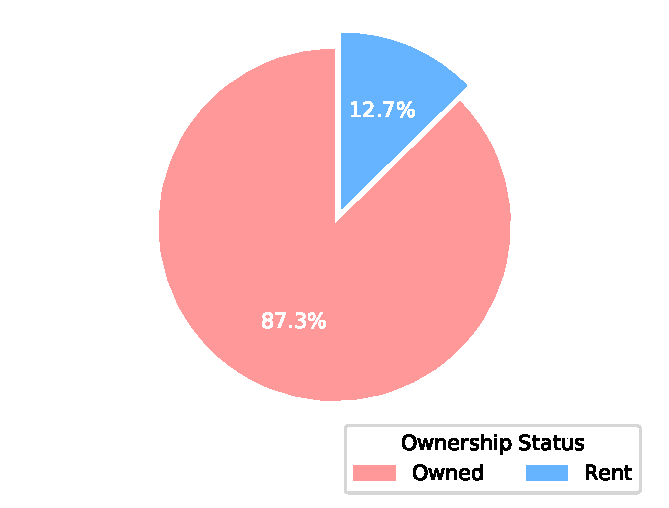
\includegraphics{index_files/figure-pdf/fig-piechartos-output-1.pdf}

}

\caption{\label{fig-piechartos}Ownership status of respondents under
study.}

\end{figure}%

\textsubscript{Source:
\href{https://sijuswamyresearch.github.io/SM-project/index.qmd.html}{Article
Notebook}}

Above figure shows the distribution of ownership (owning a home) versus
renting among the survey respondents. Here's an interpretation in the
context of a study on public readiness for smart meters:

A significant majority of respondents (87.3\%) indicated they own their
homes. This suggests the study focuses on a population segment that
might be more likely to make long-term decisions about their residences,
potentially impacting smart meter adoption. Homeownership can influence
willingness to adopt new technologies for the home. Homeowners might be
more receptive to smart meters, as they represent an investment in their
property that could lead to long-term benefits like cost savings and
improved energy efficiency. Additionally, homeowners have more control
over implementing changes within their residences, potentially
simplifying the smart meter adoption process. However, despite potential
long-term benefits, the upfront costs associated with smart meter
installation could be a barrier for some homeowners. The perceived value
proposition of smart meters needs to be effectively communicated to
homeowners to encourage adoption.

The smaller proportion of renters (12.7\%) should not be ignored.
Understanding their perspective on smart meters is also important. Smart
meter adoption in rental properties might depend on landlord decisions
and willingness to invest. Communication strategies for renters should
highlight the potential benefits they can experience with smart meters,
such as real-time monitoring of their energy consumption to identify
areas for cost savings. By addressing both homeowners and renters, the
study can provide a comprehensive understanding of public readiness for
smart meters and inform targeted communication strategies to promote
their adoption.

\begin{longtable}[]{@{}llll@{}}
\caption{Cross-tabulation of home ownership by
generation}\label{tbl-ownership-generation}\tabularnewline
\toprule\noalign{}
Ownership & Generation Z & Millennials & Total \\
\midrule\noalign{}
\endfirsthead
\toprule\noalign{}
Ownership & Generation Z & Millennials & Total \\
\midrule\noalign{}
\endhead
\bottomrule\noalign{}
\endlastfoot
Owned & 236 & 199 & 435 \\
Rent & 37 & 26 & 63 \\
Total & 273 & 225 & 498 \\
\end{longtable}

Table~\ref{tbl-ownership-generation} reveals interesting patterns in
home ownership rates between Generation Z and Millennials within the
survey. A high proportion of Gen Z respondents (86.4\%) own their homes.
This could be due to several factors, such as cultural norms around
homeownership in certain regions or inheritance and financial assistance
from older generations. A smaller portion of Gen Z rents (13.6\%),
potentially reflecting factors like early career stages where renting is
more common or pursuing education and delaying homeownership.

Millennials also show a high rate of homeownership (88.4\%). Compared to
Gen Z, a slightly higher proportion of Millennials rent (11.6\%). This
could be due to factors like a lag in homeownership due to economic
factors impacting their generation or a preference for urban living
where renting might be more common. These generational differences in
home ownership can provide valuable insights for understanding public
readiness for smart meters and tailoring communication strategies
accordingly.

\subsubsection{Home Size and Related
Data}\label{home-size-and-related-data}

Statistical summary of the built-in area (in square feet) is shown in
Table~\ref{tbl-home-size-summary}.

\begin{longtable}[]{@{}
  >{\raggedright\arraybackslash}p{(\columnwidth - 12\tabcolsep) * \real{0.1791}}
  >{\raggedright\arraybackslash}p{(\columnwidth - 12\tabcolsep) * \real{0.0746}}
  >{\raggedright\arraybackslash}p{(\columnwidth - 12\tabcolsep) * \real{0.1045}}
  >{\raggedright\arraybackslash}p{(\columnwidth - 12\tabcolsep) * \real{0.1343}}
  >{\raggedright\arraybackslash}p{(\columnwidth - 12\tabcolsep) * \real{0.1343}}
  >{\raggedright\arraybackslash}p{(\columnwidth - 12\tabcolsep) * \real{0.1343}}
  >{\raggedright\arraybackslash}p{(\columnwidth - 12\tabcolsep) * \real{0.2388}}@{}}
\caption{Statistical summary of the built-in area (in square
feet)}\label{tbl-home-size-summary}\tabularnewline
\toprule\noalign{}
\begin{minipage}[b]{\linewidth}\raggedright
Home Size
\end{minipage} & \begin{minipage}[b]{\linewidth}\raggedright
N
\end{minipage} & \begin{minipage}[b]{\linewidth}\raggedright
Range
\end{minipage} & \begin{minipage}[b]{\linewidth}\raggedright
Minimum
\end{minipage} & \begin{minipage}[b]{\linewidth}\raggedright
Maximum
\end{minipage} & \begin{minipage}[b]{\linewidth}\raggedright
Mean
\end{minipage} & \begin{minipage}[b]{\linewidth}\raggedright
Std. Deviation
\end{minipage} \\
\midrule\noalign{}
\endfirsthead
\toprule\noalign{}
\begin{minipage}[b]{\linewidth}\raggedright
Home Size
\end{minipage} & \begin{minipage}[b]{\linewidth}\raggedright
N
\end{minipage} & \begin{minipage}[b]{\linewidth}\raggedright
Range
\end{minipage} & \begin{minipage}[b]{\linewidth}\raggedright
Minimum
\end{minipage} & \begin{minipage}[b]{\linewidth}\raggedright
Maximum
\end{minipage} & \begin{minipage}[b]{\linewidth}\raggedright
Mean
\end{minipage} & \begin{minipage}[b]{\linewidth}\raggedright
Std. Deviation
\end{minipage} \\
\midrule\noalign{}
\endhead
\bottomrule\noalign{}
\endlastfoot
Home size & 498 & 11756 & 226 & 11778 & 1724.66 & 1803.627 \\
\end{longtable}

A new categorical variable is created for a more meaningful comparison.
Those homes with built-in area exceeding 2500 Sq.ft are considered as
large, between 1000 and 2500 Sq.ft as medium, and those homes less than
1000 Sq.ft as small homes. Under this categorization, the distribution
of respondent's home size is shown in
Table~\ref{tbl-home-size-distribution}.

\begin{longtable}[]{@{}
  >{\raggedright\arraybackslash}p{(\columnwidth - 8\tabcolsep) * \real{0.1791}}
  >{\raggedright\arraybackslash}p{(\columnwidth - 8\tabcolsep) * \real{0.1642}}
  >{\raggedright\arraybackslash}p{(\columnwidth - 8\tabcolsep) * \real{0.1343}}
  >{\raggedright\arraybackslash}p{(\columnwidth - 8\tabcolsep) * \real{0.2239}}
  >{\raggedright\arraybackslash}p{(\columnwidth - 8\tabcolsep) * \real{0.2985}}@{}}
\caption{Distribution of respondent's home
size}\label{tbl-home-size-distribution}\tabularnewline
\toprule\noalign{}
\begin{minipage}[b]{\linewidth}\raggedright
Home Size
\end{minipage} & \begin{minipage}[b]{\linewidth}\raggedright
Frequency
\end{minipage} & \begin{minipage}[b]{\linewidth}\raggedright
Percent
\end{minipage} & \begin{minipage}[b]{\linewidth}\raggedright
Valid Percent
\end{minipage} & \begin{minipage}[b]{\linewidth}\raggedright
Cumulative Percent
\end{minipage} \\
\midrule\noalign{}
\endfirsthead
\toprule\noalign{}
\begin{minipage}[b]{\linewidth}\raggedright
Home Size
\end{minipage} & \begin{minipage}[b]{\linewidth}\raggedright
Frequency
\end{minipage} & \begin{minipage}[b]{\linewidth}\raggedright
Percent
\end{minipage} & \begin{minipage}[b]{\linewidth}\raggedright
Valid Percent
\end{minipage} & \begin{minipage}[b]{\linewidth}\raggedright
Cumulative Percent
\end{minipage} \\
\midrule\noalign{}
\endhead
\bottomrule\noalign{}
\endlastfoot
Large & 93 & 18.7 & 18.7 & 18.7 \\
Medium & 254 & 51.0 & 51.0 & 69.7 \\
Small & 151 & 30.3 & 30.3 & 100.0 \\
Total & 498 & 100.0 & 100.0 & 100.0 \\
\end{longtable}

A cross tabulation of the home size over generation is shown in
Table~\ref{tbl-home-size-generation}.

\begin{longtable}[]{@{}llll@{}}
\caption{Cross-tabulation of home size by
generation}\label{tbl-home-size-generation}\tabularnewline
\toprule\noalign{}
House Type & Generation Z & Millennials & Total \\
\midrule\noalign{}
\endfirsthead
\toprule\noalign{}
House Type & Generation Z & Millennials & Total \\
\midrule\noalign{}
\endhead
\bottomrule\noalign{}
\endlastfoot
Large & 41 & 52 & 93 \\
Medium & 144 & 110 & 254 \\
Small & 88 & 63 & 151 \\
Total & 273 & 225 & 498 \\
\end{longtable}

This cross-tabulation sheds light on the preferred house type (size)
among Generation Z and Millennials within the survey. Across both
generations, the majority of respondents (51.0\%) prefer medium-sized
houses. However, there are some interesting differences between
generations. Generation Z (54.8\%) leans slightly towards smaller homes,
with 32.2\% preferring small houses compared to Millennials. They also
prefer medium-sized homes (52.7\%) but to a slightly lesser extent than
Millennials, and show the lowest preference for large houses (15.0\%)
among the two groups. On the other hand, Millennials (45.2\%) tend to
favor slightly larger homes, with 48.9\% preferring medium-sized homes,
28.0\% preferring small houses, and 23.1\% showing a higher preference
for large houses compared to Gen Z.

Understanding these house size preferences can be relevant when
considering smart meter adoption. House size can influence energy
consumption patterns, as larger homes generally require more energy for
heating, cooling, and powering appliances. For those preferring smaller
or medium-sized homes, it is important to highlight the potential
cost-saving benefits of smart meters in efficiently managing energy use
in compact spaces. For those preferring larger homes, emphasizing the
ability of smart meters to provide greater insights into energy
consumption across various zones within a larger living space can
facilitate targeted conservation efforts.

\subsubsection{Consumption Profile}\label{consumption-profile}

The respondent's consumption profile is shown in
Table~\ref{tbl-consumption-profile}.

\begin{longtable}[]{@{}
  >{\raggedright\arraybackslash}p{(\columnwidth - 8\tabcolsep) * \real{0.2857}}
  >{\raggedright\arraybackslash}p{(\columnwidth - 8\tabcolsep) * \real{0.1429}}
  >{\raggedright\arraybackslash}p{(\columnwidth - 8\tabcolsep) * \real{0.1169}}
  >{\raggedright\arraybackslash}p{(\columnwidth - 8\tabcolsep) * \real{0.1948}}
  >{\raggedright\arraybackslash}p{(\columnwidth - 8\tabcolsep) * \real{0.2597}}@{}}
\caption{Distribution of respondent's consumption
profile}\label{tbl-consumption-profile}\tabularnewline
\toprule\noalign{}
\begin{minipage}[b]{\linewidth}\raggedright
Consumption Profile
\end{minipage} & \begin{minipage}[b]{\linewidth}\raggedright
Frequency
\end{minipage} & \begin{minipage}[b]{\linewidth}\raggedright
Percent
\end{minipage} & \begin{minipage}[b]{\linewidth}\raggedright
Valid Percent
\end{minipage} & \begin{minipage}[b]{\linewidth}\raggedright
Cumulative Percent
\end{minipage} \\
\midrule\noalign{}
\endfirsthead
\toprule\noalign{}
\begin{minipage}[b]{\linewidth}\raggedright
Consumption Profile
\end{minipage} & \begin{minipage}[b]{\linewidth}\raggedright
Frequency
\end{minipage} & \begin{minipage}[b]{\linewidth}\raggedright
Percent
\end{minipage} & \begin{minipage}[b]{\linewidth}\raggedright
Valid Percent
\end{minipage} & \begin{minipage}[b]{\linewidth}\raggedright
Cumulative Percent
\end{minipage} \\
\midrule\noalign{}
\endhead
\bottomrule\noalign{}
\endlastfoot
Moderate & 252 & 50.6 & 50.6 & 50.6 \\
Some what Liberal & 143 & 28.7 & 28.7 & 79.3 \\
Very Liberal & 98 & 19.7 & 19.7 & 99.0 \\
Unchanging & 5 & 1.0 & 1.0 & 100.0 \\
Total & 498 & 100.0 & 100.0 & 100.0 \\
\end{longtable}

Cross tabulation of consumption profile over generation is shown in the
following table.

\begin{longtable}[]{@{}llll@{}}
\caption{Cross-tabulation of consumption profile by
generation}\label{tbl-consumption-profile-generation}\tabularnewline
\toprule\noalign{}
Consumption Profile & Generation Z & Millennials & Total \\
\midrule\noalign{}
\endfirsthead
\toprule\noalign{}
Consumption Profile & Generation Z & Millennials & Total \\
\midrule\noalign{}
\endhead
\bottomrule\noalign{}
\endlastfoot
Moderate & 149 & 103 & 252 \\
Some what Liberal & 78 & 65 & 143 \\
Unchanging & 2 & 3 & 5 \\
Very Liberal & 44 & 54 & 98 \\
Total & 273 & 225 & 498 \\
\end{longtable}

This cross-tabulation provides insights into the consumption profiles
(reported levels of consumption) of Generation Z and Millennials within
the survey. Across both generations, a majority of respondents (50.6\%)
identify with a ``Moderate'' consumption profile. However, there are
some variations in consumption tendencies between the two groups.
Generation Z (54.8\%) leans slightly more towards moderate consumption
(54.6\%). Millennials (45.2\%) show a slightly higher presence in both
ends of the spectrum, with 28.9\% identifying with ``Some what Liberal''
consumption compared to Gen Z (28.6\%), and 24.0\% falling under ``Very
Liberal'' consumption compared to Gen Z (16.1\%).

These generational consumption differences could be due to several
factors. Gen Z, likely in earlier career stages, might have lower
disposable income for discretionary spending. Millennials, potentially
more established, might prioritize experiences or environmentally
conscious consumption. Understanding these consumption profiles can
inform communication strategies for smart meter adoption. For moderate
consumers, it is important to emphasize the cost-saving benefits of
smart meters in optimizing energy use and potentially reducing bills.
For those with more liberal consumption profiles, highlighting the
ability of smart meters to track consumption patterns and identify areas
for potential reduction can align with environmentally conscious values.

\subsubsection{Consumption Profile by Home
Size}\label{consumption-profile-by-home-size}

Cross tabulation of consumption profile and the home size is shown in
Table~\ref{tbl-consumption-profile-home-size}.

\begin{longtable}[]{@{}lllll@{}}
\caption{Cross-tabulation of consumption profile by home
size}\label{tbl-consumption-profile-home-size}\tabularnewline
\toprule\noalign{}
Consumption Profile & Large & Medium & Small & Total \\
\midrule\noalign{}
\endfirsthead
\toprule\noalign{}
Consumption Profile & Large & Medium & Small & Total \\
\midrule\noalign{}
\endhead
\bottomrule\noalign{}
\endlastfoot
Moderate & 51 & 126 & 75 & 252 \\
Some what Liberal & 28 & 77 & 38 & 143 \\
Unchanging & 1 & 2 & 2 & 5 \\
Very Liberal & 13 & 49 & 36 & 98 \\
Total & 93 & 254 & 151 & 498 \\
\end{longtable}

This cross-tabulation provides insights into the consumption profiles
(reported levels of consumption) across different house sizes. A
majority across all house sizes identify with a ``Moderate'' consumption
profile. Specifically, 54.8\% of residents in large homes, 49.6\% of
residents in medium homes, and 49.7\% of residents in small homes
exhibit moderate consumption.

However, there are variations in consumption by house size. While
moderate consumption is dominant in large homes, a slightly higher
proportion leans towards ``Very Liberal'' consumption (14.0\%) compared
to other house sizes. This could be due to factors like larger living
spaces requiring more energy for amenities like pools or Jacuzzis, or
larger families with potentially higher overall consumption needs.
Medium homes show a balanced presence across all consumption profiles,
potentially reflecting a mix of family sizes and lifestyles within this
category. Small homes have a slightly lower presence in the ``Very
Liberal'' consumption category (23.8\%) compared to larger homes,
aligning with the smaller space potentially limiting high-consumption
activities.

Understanding this interplay between house size and consumption habits
can be valuable for tailoring communication strategies for smart meter
adoption. For moderate consumers across all house sizes, it is important
to emphasize the cost-saving benefits and efficient energy management
through smart meters. For large homes, highlighting functionalities like
zone-wise monitoring to identify areas of high consumption in larger
living spaces and addressing potential concerns about managing energy
use effectively with smart meters can be beneficial. Regardless of house
size or consumption profile, some might be concerned about increased
monitoring or control over energy use. Communication strategies should
address these concerns and emphasize user control over data and privacy
settings.

\subsection{Reliability of the Construct for Statistical
Analysis}\label{reliability-of-the-construct-for-statistical-analysis}

All the constructs are tested for reliability using Cronbach's alpha.
The reliability score is shown in
Table~\ref{tbl-reliability-statistics}.

\begin{longtable}[]{@{}lll@{}}
\caption{Reliability statistics for the
constructs}\label{tbl-reliability-statistics}\tabularnewline
\toprule\noalign{}
Reliability Statistics & Cronbach's Alpha & N of Items \\
\midrule\noalign{}
\endfirsthead
\toprule\noalign{}
Reliability Statistics & Cronbach's Alpha & N of Items \\
\midrule\noalign{}
\endhead
\bottomrule\noalign{}
\endlastfoot
& .717 & 10 \\
\end{longtable}

Since the Cronbach's alpha is greater than 0.7, all the constructs are
statistically reliable. Normality of the constructs is investigated
before generalizing the findings. After the Box-Cox transformation, all
the constructs are found to be sufficiently normal with the
Kolmogorov-Smirnoff's test and Shapiro-Wilk tests. For all the
constructs, the p-values are greater than 0.05.

In the next section, the self-assessment of individual energy usage is
analyzed statistically.

\subsection{Analysis of Self-assessment of Individual Energy
Usage}\label{analysis-of-self-assessment-of-individual-energy-usage}

To investigate the individual energy usage and the respondent's
willingness to optimize their energy consumption, their self-assessment
responses are taken into account.

\subsubsection{Perception of Optimized Energy
Usage}\label{perception-of-optimized-energy-usage}

The statistical summary of the perception of optimized use of energy is
shown in Table~\ref{tbl-perception-optimized-usage}.

\begin{longtable}[]{@{}
  >{\raggedright\arraybackslash}p{(\columnwidth - 12\tabcolsep) * \real{0.3678}}
  >{\raggedright\arraybackslash}p{(\columnwidth - 12\tabcolsep) * \real{0.0575}}
  >{\raggedright\arraybackslash}p{(\columnwidth - 12\tabcolsep) * \real{0.0805}}
  >{\raggedright\arraybackslash}p{(\columnwidth - 12\tabcolsep) * \real{0.1034}}
  >{\raggedright\arraybackslash}p{(\columnwidth - 12\tabcolsep) * \real{0.1034}}
  >{\raggedright\arraybackslash}p{(\columnwidth - 12\tabcolsep) * \real{0.1034}}
  >{\raggedright\arraybackslash}p{(\columnwidth - 12\tabcolsep) * \real{0.1839}}@{}}
\caption{Statistical summary of the perception of optimized energy
usage}\label{tbl-perception-optimized-usage}\tabularnewline
\toprule\noalign{}
\begin{minipage}[b]{\linewidth}\raggedright
Perception on Optimized Usage
\end{minipage} & \begin{minipage}[b]{\linewidth}\raggedright
N
\end{minipage} & \begin{minipage}[b]{\linewidth}\raggedright
Range
\end{minipage} & \begin{minipage}[b]{\linewidth}\raggedright
Minimum
\end{minipage} & \begin{minipage}[b]{\linewidth}\raggedright
Maximum
\end{minipage} & \begin{minipage}[b]{\linewidth}\raggedright
Mean
\end{minipage} & \begin{minipage}[b]{\linewidth}\raggedright
Std. Deviation
\end{minipage} \\
\midrule\noalign{}
\endfirsthead
\toprule\noalign{}
\begin{minipage}[b]{\linewidth}\raggedright
Perception on Optimized Usage
\end{minipage} & \begin{minipage}[b]{\linewidth}\raggedright
N
\end{minipage} & \begin{minipage}[b]{\linewidth}\raggedright
Range
\end{minipage} & \begin{minipage}[b]{\linewidth}\raggedright
Minimum
\end{minipage} & \begin{minipage}[b]{\linewidth}\raggedright
Maximum
\end{minipage} & \begin{minipage}[b]{\linewidth}\raggedright
Mean
\end{minipage} & \begin{minipage}[b]{\linewidth}\raggedright
Std. Deviation
\end{minipage} \\
\midrule\noalign{}
\endhead
\bottomrule\noalign{}
\endlastfoot
& 498 & 16.0 & 5.0 & 21.0 & 13.745 & 2.8773 \\
Valid N (listwise) & 498 & & & & & \\
\end{longtable}

Table~\ref{tbl-perception-optimized-usage} summarizes the statistical
information for a variable related to how respondents perceive their
ability to optimize energy use, likely measured on a five-point Likert
scale. The data includes responses from 498 participants (N = 498). The
range of scores (Range = 16.0) indicates a spread in perceptions, with
values going from a minimum of 5.0 (likely representing ``very low
ability to optimize'') to a maximum of 21.0 (likely representing ``very
high ability to optimize''). The average score is 13.745. With a
five-point Likert scale, a score around the midpoint (in this case, 15)
would suggest a neutral perception of one's ability to optimize energy
use. Since the mean falls slightly below the midpoint, it leans slightly
towards a perception of lower ability to optimize. However, the standard
deviation of 2.8773 indicates that there's still variation in these
perceptions.

It's important to consider this data alongside the high aggregate score
(25) for willingness to optimize energy use. This suggests a general
positive sentiment towards taking steps to improve energy efficiency,
even if respondents perceive their current ability to optimize as
somewhat limited. Smart meter adoption could be particularly appealing
for those who score lower on the scale, as smart meters can provide
valuable data and insights to help them achieve their energy
optimization goals.

\subsubsection{Impact of Generation on Optimized Usage
Perception}\label{impact-of-generation-on-optimized-usage-perception}

The statistical summary of the perceived optimized usage score over
generation is shown in Table~\ref{tbl-optimized-usage-generation}.

\begin{longtable}[]{@{}llll@{}}
\caption{Statistical summary of perceived optimized usage score by
generation}\label{tbl-optimized-usage-generation}\tabularnewline
\toprule\noalign{}
Class & Mean & N & Std. Deviation \\
\midrule\noalign{}
\endfirsthead
\toprule\noalign{}
Class & Mean & N & Std. Deviation \\
\midrule\noalign{}
\endhead
\bottomrule\noalign{}
\endlastfoot
Generation Z & 14.092 & 273 & 2.9147 \\
Millennials & 13.324 & 225 & 2.7801 \\
Total & 13.745 & 498 & 2.8773 \\
\end{longtable}

The data reveals interesting insights into how Generation Z and
Millennials perceive their ability to optimize energy use. Measured on a
likely five-point Likert scale, both generations scored around the
midpoint (13.745 overall), suggesting a somewhat neutral perception of
their current optimization capabilities. However, a slight generational
difference emerged. Gen Z scored slightly higher (14.092) compared to
Millennials (13.324), indicating they might feel more confident in their
existing efforts. Despite this variation, the high overall willingness
score (26) for optimizing energy use suggests a general positive
sentiment across both groups.

This positive sentiment towards optimization creates fertile ground for
promoting smart meter adoption. While Gen Z might be drawn to smart
meters as a tool to complement their existing efforts and gain further
data-driven insights, Millennials could find them particularly valuable
for empowering them to take control and achieve their energy
optimization goals.

An ANOVA test is conducted to see if Generation Z and Millennials
differed in their perception of optimized energy use. The result of the
ANOVA test to examine the significance of this difference in the mean
perception score over the generation is shown in
Table~\ref{tbl-anova-optimized-usage}.

\begin{longtable}[]{@{}
  >{\raggedright\arraybackslash}p{(\columnwidth - 10\tabcolsep) * \real{0.3099}}
  >{\raggedright\arraybackslash}p{(\columnwidth - 10\tabcolsep) * \real{0.2254}}
  >{\raggedright\arraybackslash}p{(\columnwidth - 10\tabcolsep) * \real{0.0704}}
  >{\raggedright\arraybackslash}p{(\columnwidth - 10\tabcolsep) * \real{0.1831}}
  >{\raggedright\arraybackslash}p{(\columnwidth - 10\tabcolsep) * \real{0.1127}}
  >{\raggedright\arraybackslash}p{(\columnwidth - 10\tabcolsep) * \real{0.0986}}@{}}
\caption{ANOVA table for perception of optimized energy use by
generation}\label{tbl-anova-optimized-usage}\tabularnewline
\toprule\noalign{}
\begin{minipage}[b]{\linewidth}\raggedright
Source of Variation
\end{minipage} & \begin{minipage}[b]{\linewidth}\raggedright
Sum of Squares
\end{minipage} & \begin{minipage}[b]{\linewidth}\raggedright
df
\end{minipage} & \begin{minipage}[b]{\linewidth}\raggedright
Mean Square
\end{minipage} & \begin{minipage}[b]{\linewidth}\raggedright
F
\end{minipage} & \begin{minipage}[b]{\linewidth}\raggedright
Sig.
\end{minipage} \\
\midrule\noalign{}
\endfirsthead
\toprule\noalign{}
\begin{minipage}[b]{\linewidth}\raggedright
Source of Variation
\end{minipage} & \begin{minipage}[b]{\linewidth}\raggedright
Sum of Squares
\end{minipage} & \begin{minipage}[b]{\linewidth}\raggedright
df
\end{minipage} & \begin{minipage}[b]{\linewidth}\raggedright
Mean Square
\end{minipage} & \begin{minipage}[b]{\linewidth}\raggedright
F
\end{minipage} & \begin{minipage}[b]{\linewidth}\raggedright
Sig.
\end{minipage} \\
\midrule\noalign{}
\endhead
\bottomrule\noalign{}
\endlastfoot
Between Groups & 72.586 & 1 & 72.586 & 8.907 & .003 \\
Within Groups & 4042.026 & 496 & 8.149 & & \\
Total & 4114.612 & 497 & & & \\
\end{longtable}

The results revealed a statistically significant difference (p-value =
0.003), indicating that we can reject the null hypothesis of no
difference between the generations. This suggests Generation Z and
Millennials have statistically distinct perceptions on how much energy
they use optimally.

From the statistical analysis, it is clear that both Gen Z and
Millennials are willing to reduce their current energy usage.

\subsubsection{Perspective on Sharing Consumption
Information}\label{perspective-on-sharing-consumption-information}

The smart meter facility will share details of energy consumption of the
individual customer. This aspect is studied in this research. The
statistical summary of the perception of sharing consumption information
is shown in Table~\ref{tbl-perception-sharing-info}.

\begin{longtable}[]{@{}
  >{\raggedright\arraybackslash}p{(\columnwidth - 12\tabcolsep) * \real{0.3205}}
  >{\raggedright\arraybackslash}p{(\columnwidth - 12\tabcolsep) * \real{0.0641}}
  >{\raggedright\arraybackslash}p{(\columnwidth - 12\tabcolsep) * \real{0.0897}}
  >{\raggedright\arraybackslash}p{(\columnwidth - 12\tabcolsep) * \real{0.1154}}
  >{\raggedright\arraybackslash}p{(\columnwidth - 12\tabcolsep) * \real{0.1154}}
  >{\raggedright\arraybackslash}p{(\columnwidth - 12\tabcolsep) * \real{0.0897}}
  >{\raggedright\arraybackslash}p{(\columnwidth - 12\tabcolsep) * \real{0.2051}}@{}}
\caption{Statistical summary of the perception of sharing consumption
information}\label{tbl-perception-sharing-info}\tabularnewline
\toprule\noalign{}
\begin{minipage}[b]{\linewidth}\raggedright
Descriptive Statistics
\end{minipage} & \begin{minipage}[b]{\linewidth}\raggedright
N
\end{minipage} & \begin{minipage}[b]{\linewidth}\raggedright
Range
\end{minipage} & \begin{minipage}[b]{\linewidth}\raggedright
Minimum
\end{minipage} & \begin{minipage}[b]{\linewidth}\raggedright
Maximum
\end{minipage} & \begin{minipage}[b]{\linewidth}\raggedright
Mean
\end{minipage} & \begin{minipage}[b]{\linewidth}\raggedright
Std. Deviation
\end{minipage} \\
\midrule\noalign{}
\endfirsthead
\toprule\noalign{}
\begin{minipage}[b]{\linewidth}\raggedright
Descriptive Statistics
\end{minipage} & \begin{minipage}[b]{\linewidth}\raggedright
N
\end{minipage} & \begin{minipage}[b]{\linewidth}\raggedright
Range
\end{minipage} & \begin{minipage}[b]{\linewidth}\raggedright
Minimum
\end{minipage} & \begin{minipage}[b]{\linewidth}\raggedright
Maximum
\end{minipage} & \begin{minipage}[b]{\linewidth}\raggedright
Mean
\end{minipage} & \begin{minipage}[b]{\linewidth}\raggedright
Std. Deviation
\end{minipage} \\
\midrule\noalign{}
\endhead
\bottomrule\noalign{}
\endlastfoot
Perception on Sharing Consumption Information & 498 & 12 & 2 & 14 &
10.22 & 2.581 \\
Valid N (listwise) & 498 & & & & & \\
\end{longtable}

This table summarizes the statistical information for a variable related
to respondents' willingness to share information on their energy
consumption. The data includes responses from 498 participants (N =
498). The range of scores (Range = 12, minimum of 2, maximum of 14)
indicates a spread in perceptions. A higher score suggests a greater
willingness to share information. The average score of 10.22 falls
slightly below the midpoint (which would be 7 in a six-point scale),
suggesting a tendency towards being somewhat comfortable with sharing
information on energy consumption. However, the standard deviation of
2.581 indicates that there's still variation in these perceptions. Some
respondents might be very open to sharing (scoring high), while others
might be less comfortable (scoring lower).

\subsubsection{Impact of Generation on the Perception of Willingness to
Share Consumption
Information}\label{impact-of-generation-on-the-perception-of-willingness-to-share-consumption-information}

The result of comparing the mean perception score over generation is
shown in Table~\ref{tbl-sharing-info-generation}.

\begin{longtable}[]{@{}llll@{}}
\caption{Statistical summary of perceived willingness to share
consumption information by
generation}\label{tbl-sharing-info-generation}\tabularnewline
\toprule\noalign{}
Class & Mean & N & Std. Deviation \\
\midrule\noalign{}
\endfirsthead
\toprule\noalign{}
Class & Mean & N & Std. Deviation \\
\midrule\noalign{}
\endhead
\bottomrule\noalign{}
\endlastfoot
Generation Z & 10.34 & 273 & 2.592 \\
Millennials & 10.08 & 225 & 2.566 \\
Total & 10.22 & 498 & 2.581 \\
\end{longtable}

There's a slight generational difference in willingness to share
information on energy consumption. Generation Z scored slightly higher
(mean = 10.34) than Millennials (mean = 10.08) on a scale likely ranging
from 2 (least willing) to 14 (most willing). However, the standard
deviations (around 2.6) for both groups indicate a spread of opinions
within each generation. This suggests that a one-size-fits-all
communication strategy might not be the most effective. For both
generations, addressing potential privacy concerns around data sharing
will be important. Additionally, considering generational nuances could
be beneficial. Highlighting how smart meters can complement existing
efforts and provide data-driven insights might resonate more with Gen Z,
whereas emphasizing smart meters as a tool for taking control and
achieving energy goals could be more impactful for Millennials.

An Analysis of Variance (ANOVA) is conducted to assess if Generation Z
and Millennials differed statistically in their willingness to share
information on energy consumption. The result of the ANOVA test is shown
in Table~\ref{tbl-anova-sharing-info}.

\begin{longtable}[]{@{}
  >{\raggedright\arraybackslash}p{(\columnwidth - 10\tabcolsep) * \real{0.3099}}
  >{\raggedright\arraybackslash}p{(\columnwidth - 10\tabcolsep) * \real{0.2254}}
  >{\raggedright\arraybackslash}p{(\columnwidth - 10\tabcolsep) * \real{0.0704}}
  >{\raggedright\arraybackslash}p{(\columnwidth - 10\tabcolsep) * \real{0.1831}}
  >{\raggedright\arraybackslash}p{(\columnwidth - 10\tabcolsep) * \real{0.1127}}
  >{\raggedright\arraybackslash}p{(\columnwidth - 10\tabcolsep) * \real{0.0986}}@{}}
\caption{ANOVA table for willingness to share consumption information by
generation}\label{tbl-anova-sharing-info}\tabularnewline
\toprule\noalign{}
\begin{minipage}[b]{\linewidth}\raggedright
Source of Variation
\end{minipage} & \begin{minipage}[b]{\linewidth}\raggedright
Sum of Squares
\end{minipage} & \begin{minipage}[b]{\linewidth}\raggedright
df
\end{minipage} & \begin{minipage}[b]{\linewidth}\raggedright
Mean Square
\end{minipage} & \begin{minipage}[b]{\linewidth}\raggedright
F
\end{minipage} & \begin{minipage}[b]{\linewidth}\raggedright
Sig.
\end{minipage} \\
\midrule\noalign{}
\endfirsthead
\toprule\noalign{}
\begin{minipage}[b]{\linewidth}\raggedright
Source of Variation
\end{minipage} & \begin{minipage}[b]{\linewidth}\raggedright
Sum of Squares
\end{minipage} & \begin{minipage}[b]{\linewidth}\raggedright
df
\end{minipage} & \begin{minipage}[b]{\linewidth}\raggedright
Mean Square
\end{minipage} & \begin{minipage}[b]{\linewidth}\raggedright
F
\end{minipage} & \begin{minipage}[b]{\linewidth}\raggedright
Sig.
\end{minipage} \\
\midrule\noalign{}
\endhead
\bottomrule\noalign{}
\endlastfoot
Between Groups & 8.380 & 1 & 8.380 & 1.259 & .262 \\
Within Groups & 3301.879 & 496 & 6.657 & & \\
Total & 3310.259 & 497 & & & \\
\end{longtable}

The null hypothesis (H0) stated there's no significant difference
between the generations. The alternative hypothesis (Ha) stated there is
a difference. The ANOVA table reveals an F-statistic of 1.259 with a
significance level (p-value) of 0.262. Since the p-value (0.262) is
greater than the commonly used significance level of 0.05, we fail to
reject the null hypothesis. This suggests there's not enough statistical
evidence to conclude a significant difference between Generation Z and
Millennials in their willingness to share consumption information.

\subsubsection{Perspective of Load Control of Residential Home by
Utility}\label{perspective-of-load-control-of-residential-home-by-utility}

The statistical summary of the perception score is shown in
Table~\ref{tbl-perception-load-control}.

\begin{longtable}[]{@{}
  >{\raggedright\arraybackslash}p{(\columnwidth - 12\tabcolsep) * \real{0.3117}}
  >{\raggedright\arraybackslash}p{(\columnwidth - 12\tabcolsep) * \real{0.0649}}
  >{\raggedright\arraybackslash}p{(\columnwidth - 12\tabcolsep) * \real{0.0909}}
  >{\raggedright\arraybackslash}p{(\columnwidth - 12\tabcolsep) * \real{0.1169}}
  >{\raggedright\arraybackslash}p{(\columnwidth - 12\tabcolsep) * \real{0.1169}}
  >{\raggedright\arraybackslash}p{(\columnwidth - 12\tabcolsep) * \real{0.0909}}
  >{\raggedright\arraybackslash}p{(\columnwidth - 12\tabcolsep) * \real{0.2078}}@{}}
\caption{Statistical summary of the perception of load control by
utility}\label{tbl-perception-load-control}\tabularnewline
\toprule\noalign{}
\begin{minipage}[b]{\linewidth}\raggedright
Descriptive Statistics
\end{minipage} & \begin{minipage}[b]{\linewidth}\raggedright
N
\end{minipage} & \begin{minipage}[b]{\linewidth}\raggedright
Range
\end{minipage} & \begin{minipage}[b]{\linewidth}\raggedright
Minimum
\end{minipage} & \begin{minipage}[b]{\linewidth}\raggedright
Maximum
\end{minipage} & \begin{minipage}[b]{\linewidth}\raggedright
Mean
\end{minipage} & \begin{minipage}[b]{\linewidth}\raggedright
Std. Deviation
\end{minipage} \\
\midrule\noalign{}
\endfirsthead
\toprule\noalign{}
\begin{minipage}[b]{\linewidth}\raggedright
Descriptive Statistics
\end{minipage} & \begin{minipage}[b]{\linewidth}\raggedright
N
\end{minipage} & \begin{minipage}[b]{\linewidth}\raggedright
Range
\end{minipage} & \begin{minipage}[b]{\linewidth}\raggedright
Minimum
\end{minipage} & \begin{minipage}[b]{\linewidth}\raggedright
Maximum
\end{minipage} & \begin{minipage}[b]{\linewidth}\raggedright
Mean
\end{minipage} & \begin{minipage}[b]{\linewidth}\raggedright
Std. Deviation
\end{minipage} \\
\midrule\noalign{}
\endhead
\bottomrule\noalign{}
\endlastfoot
Perception on Load Control-Incentivised & 498 & 21 & 4 & 25 & 14.90 &
5.359 \\
Valid N (listwise) & 498 & & & & & \\
\end{longtable}

Table~\ref{tbl-perception-load-control} explores how comfortable people
are with load control programs that incentivize reduced energy use
during peak hours. Based on responses from 498 participants (N = 498),
the data reveals a spread of opinions on a five-point Likert scale
(range of 21 points). The average score of 14.90 suggests a tendency
towards a somewhat positive perception, though it falls slightly below
the midpoint. However, the high standard deviation of 5.359 indicates
significant variation in these perceptions. Some might be enthusiastic
about potential cost savings or environmental benefits (scoring high),
while others might have concerns about surrendering control during peak
hours (scoring lower). This highlights the need for communication
strategies that address potential concerns and clearly explain program
structure, while also emphasizing benefits like cost savings and
environmental impact reduction, to encourage wider participation and
achieve energy-saving goals.

\paragraph{Impact of Generation on the Perception of Load Control for
Residential Home by
Utility}\label{impact-of-generation-on-the-perception-of-load-control-for-residential-home-by-utility}

The summary statistics of load control perception score over generation
is shown in Table~\ref{tbl-load-control-generation}.

\begin{longtable}[]{@{}llll@{}}
\caption{Statistical summary of perceived load control by
generation}\label{tbl-load-control-generation}\tabularnewline
\toprule\noalign{}
Class & Mean & N & Std. Deviation \\
\midrule\noalign{}
\endfirsthead
\toprule\noalign{}
Class & Mean & N & Std. Deviation \\
\midrule\noalign{}
\endhead
\bottomrule\noalign{}
\endlastfoot
Generation Z & 15.33 & 273 & 5.219 \\
Millennials & 14.39 & 225 & 5.492 \\
Total & 14.90 & 498 & 5.359 \\
\end{longtable}

There's a slight generational difference in how receptive people are to
load control programs with incentives. Generation Z scored slightly
higher (mean = 15.33) than Millennials (mean = 14.39) on a five-point
Likert scale. However, the standard deviations for both groups (around
5.2-5.5) indicate a spread of opinions within each generation. This
suggests a one-size-fits-all approach for promoting these programs might
not be the most effective.

An Analysis of Variance (ANOVA) was conducted to assess if Generation Z
and Millennials differed statistically in their perception of these
programs. The null hypothesis (H0) stated there's no significant
difference between the generations. The alternative hypothesis (Ha)
stated there is a difference. The result of ANOVA is shown in
Table~\ref{tbl-anova-load-control}.

\begin{longtable}[]{@{}
  >{\raggedright\arraybackslash}p{(\columnwidth - 10\tabcolsep) * \real{0.3099}}
  >{\raggedright\arraybackslash}p{(\columnwidth - 10\tabcolsep) * \real{0.2254}}
  >{\raggedright\arraybackslash}p{(\columnwidth - 10\tabcolsep) * \real{0.0704}}
  >{\raggedright\arraybackslash}p{(\columnwidth - 10\tabcolsep) * \real{0.1831}}
  >{\raggedright\arraybackslash}p{(\columnwidth - 10\tabcolsep) * \real{0.1127}}
  >{\raggedright\arraybackslash}p{(\columnwidth - 10\tabcolsep) * \real{0.0986}}@{}}
\caption{ANOVA table for perception of load control by
generation}\label{tbl-anova-load-control}\tabularnewline
\toprule\noalign{}
\begin{minipage}[b]{\linewidth}\raggedright
Source of Variation
\end{minipage} & \begin{minipage}[b]{\linewidth}\raggedright
Sum of Squares
\end{minipage} & \begin{minipage}[b]{\linewidth}\raggedright
df
\end{minipage} & \begin{minipage}[b]{\linewidth}\raggedright
Mean Square
\end{minipage} & \begin{minipage}[b]{\linewidth}\raggedright
F
\end{minipage} & \begin{minipage}[b]{\linewidth}\raggedright
Sig.
\end{minipage} \\
\midrule\noalign{}
\endfirsthead
\toprule\noalign{}
\begin{minipage}[b]{\linewidth}\raggedright
Source of Variation
\end{minipage} & \begin{minipage}[b]{\linewidth}\raggedright
Sum of Squares
\end{minipage} & \begin{minipage}[b]{\linewidth}\raggedright
df
\end{minipage} & \begin{minipage}[b]{\linewidth}\raggedright
Mean Square
\end{minipage} & \begin{minipage}[b]{\linewidth}\raggedright
F
\end{minipage} & \begin{minipage}[b]{\linewidth}\raggedright
Sig.
\end{minipage} \\
\midrule\noalign{}
\endhead
\bottomrule\noalign{}
\endlastfoot
Between Groups & 109.684 & 1 & 109.684 & 3.841 & .051 \\
Within Groups & 14163.690 & 496 & 28.556 & & \\
Total & 14273.373 & 497 & & & \\
\end{longtable}

Table~\ref{tbl-anova-load-control} reveals a F-statistic of 3.841 with a
significance level (p-value) of 0.051. Since the p-value (0.051) is
marginally greater than the commonly used significance level of 0.05,
the results are inconclusive. We can't definitively reject the null
hypothesis, meaning there's weak evidence to suggest a statistically
significant difference between Generation Z and Millennials in their
perception of load control programs with incentives.

While the average scores suggest a slight difference (Gen Z: 15.33,
Millennials: 14.39) and the F-statistic shows some variation between
groups, the p-value doesn't provide strong enough evidence to
definitively conclude a statistically significant generational
difference.

\subsubsection{Perspectives towards Smart Grid Functions and Smart Grid
Technologies}\label{perspectives-towards-smart-grid-functions-and-smart-grid-technologies}

The statistical summary of the perception score is shown in
Table~\ref{tbl-perception-smart-grid}.

\begin{longtable}[]{@{}
  >{\raggedright\arraybackslash}p{(\columnwidth - 10\tabcolsep) * \real{0.3521}}
  >{\raggedright\arraybackslash}p{(\columnwidth - 10\tabcolsep) * \real{0.0704}}
  >{\raggedright\arraybackslash}p{(\columnwidth - 10\tabcolsep) * \real{0.1268}}
  >{\raggedright\arraybackslash}p{(\columnwidth - 10\tabcolsep) * \real{0.1268}}
  >{\raggedright\arraybackslash}p{(\columnwidth - 10\tabcolsep) * \real{0.0986}}
  >{\raggedright\arraybackslash}p{(\columnwidth - 10\tabcolsep) * \real{0.2254}}@{}}
\caption{Statistical summary of the perception of smart grid
technologies}\label{tbl-perception-smart-grid}\tabularnewline
\toprule\noalign{}
\begin{minipage}[b]{\linewidth}\raggedright
Descriptive Statistics
\end{minipage} & \begin{minipage}[b]{\linewidth}\raggedright
N
\end{minipage} & \begin{minipage}[b]{\linewidth}\raggedright
Minimum
\end{minipage} & \begin{minipage}[b]{\linewidth}\raggedright
Maximum
\end{minipage} & \begin{minipage}[b]{\linewidth}\raggedright
Mean
\end{minipage} & \begin{minipage}[b]{\linewidth}\raggedright
Std. Deviation
\end{minipage} \\
\midrule\noalign{}
\endfirsthead
\toprule\noalign{}
\begin{minipage}[b]{\linewidth}\raggedright
Descriptive Statistics
\end{minipage} & \begin{minipage}[b]{\linewidth}\raggedright
N
\end{minipage} & \begin{minipage}[b]{\linewidth}\raggedright
Minimum
\end{minipage} & \begin{minipage}[b]{\linewidth}\raggedright
Maximum
\end{minipage} & \begin{minipage}[b]{\linewidth}\raggedright
Mean
\end{minipage} & \begin{minipage}[b]{\linewidth}\raggedright
Std. Deviation
\end{minipage} \\
\midrule\noalign{}
\endhead
\bottomrule\noalign{}
\endlastfoot
Perception on Smart Grid & 498 & 0 & 22 & 13.80 & 7.496 \\
Valid N (listwise) & 498 & & & & \\
\end{longtable}

This table summarizes how comfortable people are with smart grids,
likely measured using five Likert-scaled items on a construct related to
the technology (N = 498). The range of scores (0 to 25) indicates a
broad spectrum of opinions. The average score of 13.80, with a maximum
possible score of 25, suggests a perception that leans closer to neutral
on smart grids. However, the high standard deviation of 7.496 highlights
a significant variation in these perceptions. Some respondents might be
very enthusiastic about smart grids (scoring high), while others might
have reservations or limited understanding (scoring lower).

\paragraph{Impact of Generation on the Perception Score of Smart
Grid}\label{impact-of-generation-on-the-perception-score-of-smart-grid}

The statistical summary of smart grid perception score over generation
is shown in Table~\ref{tbl-smart-grid-generation}.

\begin{longtable}[]{@{}llll@{}}
\caption{Statistical summary of perceived smart grid technologies by
generation}\label{tbl-smart-grid-generation}\tabularnewline
\toprule\noalign{}
Class & Mean & N & Std. Deviation \\
\midrule\noalign{}
\endfirsthead
\toprule\noalign{}
Class & Mean & N & Std. Deviation \\
\midrule\noalign{}
\endhead
\bottomrule\noalign{}
\endlastfoot
Generation Z & 14.40 & 273 & 7.311 \\
Millennials & 13.07 & 225 & 7.669 \\
Total & 13.80 & 498 & 7.496 \\
\end{longtable}

There's a generational difference in how people view smart grids.
Generation Z scored slightly higher (mean = 14.40) than Millennials
(mean = 13.07) on a five-point Likert scale likely ranging from 0 (very
negative perception) to 25 (very positive perception). The standard
deviations (around 7.3-7.7) for both groups indicate a spread of
opinions within each generation. This suggests a one-size-fits-all
approach for promoting smart grids might not be the most effective.

An Analysis of Variance (ANOVA) is conducted to assess if Generation Z
and Millennials differed statistically in their perception of smart
grids. The null hypothesis (H0) stated there's no significant difference
between the generations. The alternative hypothesis (Ha) stated there is
a difference. The result of the ANOVA test is shown in
Table~\ref{tbl-anova-smart-grid}.

\begin{longtable}[]{@{}
  >{\raggedright\arraybackslash}p{(\columnwidth - 10\tabcolsep) * \real{0.3099}}
  >{\raggedright\arraybackslash}p{(\columnwidth - 10\tabcolsep) * \real{0.2254}}
  >{\raggedright\arraybackslash}p{(\columnwidth - 10\tabcolsep) * \real{0.0704}}
  >{\raggedright\arraybackslash}p{(\columnwidth - 10\tabcolsep) * \real{0.1831}}
  >{\raggedright\arraybackslash}p{(\columnwidth - 10\tabcolsep) * \real{0.1127}}
  >{\raggedright\arraybackslash}p{(\columnwidth - 10\tabcolsep) * \real{0.0986}}@{}}
\caption{ANOVA table for perception of smart grid technologies by
generation}\label{tbl-anova-smart-grid}\tabularnewline
\toprule\noalign{}
\begin{minipage}[b]{\linewidth}\raggedright
Source of Variation
\end{minipage} & \begin{minipage}[b]{\linewidth}\raggedright
Sum of Squares
\end{minipage} & \begin{minipage}[b]{\linewidth}\raggedright
df
\end{minipage} & \begin{minipage}[b]{\linewidth}\raggedright
Mean Square
\end{minipage} & \begin{minipage}[b]{\linewidth}\raggedright
F
\end{minipage} & \begin{minipage}[b]{\linewidth}\raggedright
Sig.
\end{minipage} \\
\midrule\noalign{}
\endfirsthead
\toprule\noalign{}
\begin{minipage}[b]{\linewidth}\raggedright
Source of Variation
\end{minipage} & \begin{minipage}[b]{\linewidth}\raggedright
Sum of Squares
\end{minipage} & \begin{minipage}[b]{\linewidth}\raggedright
df
\end{minipage} & \begin{minipage}[b]{\linewidth}\raggedright
Mean Square
\end{minipage} & \begin{minipage}[b]{\linewidth}\raggedright
F
\end{minipage} & \begin{minipage}[b]{\linewidth}\raggedright
Sig.
\end{minipage} \\
\midrule\noalign{}
\endhead
\bottomrule\noalign{}
\endlastfoot
Between Groups & 216.379 & 1 & 216.379 & 12.873 & .030 \\
Within Groups & 27712.137 & 496 & 55.871 & & \\
Total & 27928.516 & 497 & & & \\
\end{longtable}

The ANOVA table reveals an F-statistic of 12.873 with a significance
level (p-value) of 0.030. Since the p-value (0.030) is less than the
commonly used significance level of 0.05, we reject the null hypothesis.
This indicates there's statistically significant evidence to suggest a
difference in how Generation Z and Millennials perceive smart grids. The
average scores (Gen Z: 14.40, Millennials: 13.07) support this finding,
suggesting a generational difference.

\subsubsection{Perspective on Rooftop PV \& Electric
Vehicles}\label{perspective-on-rooftop-pv-electric-vehicles}

The statistical summary of the perception score on rooftop PV and EVs is
shown in Table~\ref{tbl-perception-rooftop-pv-ev}.

\begin{longtable}[]{@{}
  >{\raggedright\arraybackslash}p{(\columnwidth - 10\tabcolsep) * \real{0.3521}}
  >{\raggedright\arraybackslash}p{(\columnwidth - 10\tabcolsep) * \real{0.0704}}
  >{\raggedright\arraybackslash}p{(\columnwidth - 10\tabcolsep) * \real{0.1268}}
  >{\raggedright\arraybackslash}p{(\columnwidth - 10\tabcolsep) * \real{0.1268}}
  >{\raggedright\arraybackslash}p{(\columnwidth - 10\tabcolsep) * \real{0.0986}}
  >{\raggedright\arraybackslash}p{(\columnwidth - 10\tabcolsep) * \real{0.2254}}@{}}
\caption{Statistical summary of the perception of rooftop PV and
EVs}\label{tbl-perception-rooftop-pv-ev}\tabularnewline
\toprule\noalign{}
\begin{minipage}[b]{\linewidth}\raggedright
Descriptive Statistics
\end{minipage} & \begin{minipage}[b]{\linewidth}\raggedright
N
\end{minipage} & \begin{minipage}[b]{\linewidth}\raggedright
Minimum
\end{minipage} & \begin{minipage}[b]{\linewidth}\raggedright
Maximum
\end{minipage} & \begin{minipage}[b]{\linewidth}\raggedright
Mean
\end{minipage} & \begin{minipage}[b]{\linewidth}\raggedright
Std. Deviation
\end{minipage} \\
\midrule\noalign{}
\endfirsthead
\toprule\noalign{}
\begin{minipage}[b]{\linewidth}\raggedright
Descriptive Statistics
\end{minipage} & \begin{minipage}[b]{\linewidth}\raggedright
N
\end{minipage} & \begin{minipage}[b]{\linewidth}\raggedright
Minimum
\end{minipage} & \begin{minipage}[b]{\linewidth}\raggedright
Maximum
\end{minipage} & \begin{minipage}[b]{\linewidth}\raggedright
Mean
\end{minipage} & \begin{minipage}[b]{\linewidth}\raggedright
Std. Deviation
\end{minipage} \\
\midrule\noalign{}
\endhead
\bottomrule\noalign{}
\endlastfoot
Perception on Rooftop PV and EV & 498 & 5 & 19 & 13.96 & 3.629 \\
Valid N (listwise) & 498 & & & & \\
\end{longtable}

Table~\ref{tbl-perception-rooftop-pv-ev} summarizes how comfortable
people are with rooftop solar PV systems and electric vehicles (EVs),
likely measured using five Likert-scaled items on a construct related to
these technologies (N = 498). The range of scores (5 to 19) indicates a
spread of opinions. The average score of 13.96, with a maximum possible
score of 25, suggests a tendency towards a somewhat positive perception
of rooftop solar PV and EVs. However, the standard deviation of 3.629
highlights a moderate level of variation in these perceptions. Some
respondents might be very enthusiastic about the potential of these
technologies (scoring high), while others might have a more neutral view
(scoring lower).

\paragraph{Impact of Generation on the Perception of Rooftop PV and
EVs}\label{impact-of-generation-on-the-perception-of-rooftop-pv-and-evs}

The statistical summary of perception score on rooftop PV and EVs over
generation is shown in Table~\ref{tbl-rooftop-pv-ev-generation}.

\begin{longtable}[]{@{}llll@{}}
\caption{Statistical summary of perceived rooftop PV and EVs by
generation}\label{tbl-rooftop-pv-ev-generation}\tabularnewline
\toprule\noalign{}
Class & Mean & N & Std. Deviation \\
\midrule\noalign{}
\endfirsthead
\toprule\noalign{}
Class & Mean & N & Std. Deviation \\
\midrule\noalign{}
\endhead
\bottomrule\noalign{}
\endlastfoot
Generation Z & 13.72 & 273 & 3.724 \\
Millennials & 14.25 & 225 & 3.495 \\
Total & 13.96 & 498 & 3.629 \\
\end{longtable}

There's a slight generational difference in how people view rooftop
solar PV and EVs. Millennials scored slightly higher (mean = 14.25) than
Generation Z (mean = 13.72) on a five-point Likert scale likely ranging
from 1 (strongly disagree) to 5 (strongly agree). The standard
deviations for both groups (around 3.5-3.7) indicate a spread of
opinions within each generation. This suggests a one-size-fits-all
approach for promoting rooftop solar and EVs might not be the most
effective.

An Analysis of Variance (ANOVA) is conducted to assess if Generation Z
and Millennials differed statistically in their perception of rooftop
solar PV and EVs. The null hypothesis (H0) stated there's no significant
difference between the generations. The alternative hypothesis (Ha)
stated there is a difference. The result of the ANOVA test is shown in
Table~\ref{tbl-anova-rooftop-pv-ev}.

\begin{longtable}[]{@{}
  >{\raggedright\arraybackslash}p{(\columnwidth - 10\tabcolsep) * \real{0.3099}}
  >{\raggedright\arraybackslash}p{(\columnwidth - 10\tabcolsep) * \real{0.2254}}
  >{\raggedright\arraybackslash}p{(\columnwidth - 10\tabcolsep) * \real{0.0704}}
  >{\raggedright\arraybackslash}p{(\columnwidth - 10\tabcolsep) * \real{0.1831}}
  >{\raggedright\arraybackslash}p{(\columnwidth - 10\tabcolsep) * \real{0.1127}}
  >{\raggedright\arraybackslash}p{(\columnwidth - 10\tabcolsep) * \real{0.0986}}@{}}
\caption{ANOVA table for perception of rooftop PV and EVs by
generation}\label{tbl-anova-rooftop-pv-ev}\tabularnewline
\toprule\noalign{}
\begin{minipage}[b]{\linewidth}\raggedright
Source of Variation
\end{minipage} & \begin{minipage}[b]{\linewidth}\raggedright
Sum of Squares
\end{minipage} & \begin{minipage}[b]{\linewidth}\raggedright
df
\end{minipage} & \begin{minipage}[b]{\linewidth}\raggedright
Mean Square
\end{minipage} & \begin{minipage}[b]{\linewidth}\raggedright
F
\end{minipage} & \begin{minipage}[b]{\linewidth}\raggedright
Sig.
\end{minipage} \\
\midrule\noalign{}
\endfirsthead
\toprule\noalign{}
\begin{minipage}[b]{\linewidth}\raggedright
Source of Variation
\end{minipage} & \begin{minipage}[b]{\linewidth}\raggedright
Sum of Squares
\end{minipage} & \begin{minipage}[b]{\linewidth}\raggedright
df
\end{minipage} & \begin{minipage}[b]{\linewidth}\raggedright
Mean Square
\end{minipage} & \begin{minipage}[b]{\linewidth}\raggedright
F
\end{minipage} & \begin{minipage}[b]{\linewidth}\raggedright
Sig.
\end{minipage} \\
\midrule\noalign{}
\endhead
\bottomrule\noalign{}
\endlastfoot
Between Groups & 34.873 & 1 & 34.873 & 2.657 & .104 \\
Within Groups & 6509.402 & 496 & 13.124 & & \\
Total & 6544.275 & 497 & & & \\
\end{longtable}

The ANOVA table reveals an F-statistic of 2.657 with a significance
level (p-value) of 0.104. Since the p-value (0.104) is greater than the
commonly used significance level of 0.05, we fail to reject the null
hypothesis. This suggests there's not enough statistical evidence to
conclude a significant difference between Generation Z and Millennials
in their perception of rooftop solar PV and EVs.

While the average scores (Gen Z: 13.72, Millennials: 14.25) show a
slight difference, the ANOVA result indicates this difference is likely
due to chance and may not be statistically meaningful. It's possible
that both generations hold generally similar perceptions of rooftop
solar PV and EVs.

\subsubsection{Perspection Towards Adopting Vehicle to Grid
(V2G)}\label{perspection-towards-adopting-vehicle-to-grid-v2g}

The statistical summary of the perception score towards adopting vehicle
to grid technology is shown in Table~\ref{tbl-perception-v2g}.

\begin{longtable}[]{@{}
  >{\raggedright\arraybackslash}p{(\columnwidth - 10\tabcolsep) * \real{0.3521}}
  >{\raggedright\arraybackslash}p{(\columnwidth - 10\tabcolsep) * \real{0.0704}}
  >{\raggedright\arraybackslash}p{(\columnwidth - 10\tabcolsep) * \real{0.1268}}
  >{\raggedright\arraybackslash}p{(\columnwidth - 10\tabcolsep) * \real{0.1268}}
  >{\raggedright\arraybackslash}p{(\columnwidth - 10\tabcolsep) * \real{0.0986}}
  >{\raggedright\arraybackslash}p{(\columnwidth - 10\tabcolsep) * \real{0.2254}}@{}}
\caption{Statistical summary of the perception of vehicle to grid
technology}\label{tbl-perception-v2g}\tabularnewline
\toprule\noalign{}
\begin{minipage}[b]{\linewidth}\raggedright
Descriptive Statistics
\end{minipage} & \begin{minipage}[b]{\linewidth}\raggedright
N
\end{minipage} & \begin{minipage}[b]{\linewidth}\raggedright
Minimum
\end{minipage} & \begin{minipage}[b]{\linewidth}\raggedright
Maximum
\end{minipage} & \begin{minipage}[b]{\linewidth}\raggedright
Mean
\end{minipage} & \begin{minipage}[b]{\linewidth}\raggedright
Std. Deviation
\end{minipage} \\
\midrule\noalign{}
\endfirsthead
\toprule\noalign{}
\begin{minipage}[b]{\linewidth}\raggedright
Descriptive Statistics
\end{minipage} & \begin{minipage}[b]{\linewidth}\raggedright
N
\end{minipage} & \begin{minipage}[b]{\linewidth}\raggedright
Minimum
\end{minipage} & \begin{minipage}[b]{\linewidth}\raggedright
Maximum
\end{minipage} & \begin{minipage}[b]{\linewidth}\raggedright
Mean
\end{minipage} & \begin{minipage}[b]{\linewidth}\raggedright
Std. Deviation
\end{minipage} \\
\midrule\noalign{}
\endhead
\bottomrule\noalign{}
\endlastfoot
Perception on Vehicle to Grid & 498 & 6 & 30 & 21.27 & 4.446 \\
Valid N (listwise) & 498 & & & & \\
\end{longtable}

Table~\ref{tbl-perception-v2g} explores people's perception of V2G
technology, likely measured using the sum of scores from six, five-point
Likert-scaled attributes (N = 498). The range of scores (6 to 30)
indicates a spread of opinions. The average score is 21.27. Since the
maximum possible score is 30 (assuming all attributes received the
highest score of 5), this suggests a tendency towards a positive
perception of V2G technology. However, the standard deviation of 4.446
highlights a moderate level of variation in these perceptions.

\paragraph{Impact of Generation on the Perception Towards Adoption of
V2G
Technology}\label{impact-of-generation-on-the-perception-towards-adoption-of-v2g-technology}

The statistical summary of perception score towards the adoption of V2G
technology over the generation is shown in
Table~\ref{tbl-v2g-generation}.

\begin{longtable}[]{@{}llll@{}}
\caption{Statistical summary of perceived vehicle to grid technology by
generation}\label{tbl-v2g-generation}\tabularnewline
\toprule\noalign{}
Class & Mean & N & Std. Deviation \\
\midrule\noalign{}
\endfirsthead
\toprule\noalign{}
Class & Mean & N & Std. Deviation \\
\midrule\noalign{}
\endhead
\bottomrule\noalign{}
\endlastfoot
Generation Z & 21.10 & 273 & 4.321 \\
Millennials & 21.47 & 225 & 4.595 \\
Total & 21.27 & 498 & 4.446 \\
\end{longtable}

There's a minor generational difference in perception of V2G technology.
Millennials scored slightly higher (mean = 21.47) than Generation Z
(mean = 21.10) on a scale likely ranging from 6 (least positive
perception) to 30 (most positive perception), based on the sum of scores
from six, five-point Likert-scaled attributes. The standard deviations
for both groups (around 4.3-4.6) indicate a spread of opinions within
each generation. This suggests a one-size-fits-all approach for
promoting V2G technology might not be ideal.

An Analysis of Variance (ANOVA) is conducted to assess if Generation Z
and Millennials differed statistically in their perception of V2G
technology. The null hypothesis (H0) stated there's no significant
difference between the generations. The alternative hypothesis (Ha)
stated there is a difference. The result of the ANOVA test is shown in
Table~\ref{tbl-anova-v2g}.

\begin{longtable}[]{@{}
  >{\raggedright\arraybackslash}p{(\columnwidth - 10\tabcolsep) * \real{0.3099}}
  >{\raggedright\arraybackslash}p{(\columnwidth - 10\tabcolsep) * \real{0.2254}}
  >{\raggedright\arraybackslash}p{(\columnwidth - 10\tabcolsep) * \real{0.0704}}
  >{\raggedright\arraybackslash}p{(\columnwidth - 10\tabcolsep) * \real{0.1831}}
  >{\raggedright\arraybackslash}p{(\columnwidth - 10\tabcolsep) * \real{0.1127}}
  >{\raggedright\arraybackslash}p{(\columnwidth - 10\tabcolsep) * \real{0.0986}}@{}}
\caption{ANOVA table for perception of vehicle to grid technology by
generation}\label{tbl-anova-v2g}\tabularnewline
\toprule\noalign{}
\begin{minipage}[b]{\linewidth}\raggedright
Source of Variation
\end{minipage} & \begin{minipage}[b]{\linewidth}\raggedright
Sum of Squares
\end{minipage} & \begin{minipage}[b]{\linewidth}\raggedright
df
\end{minipage} & \begin{minipage}[b]{\linewidth}\raggedright
Mean Square
\end{minipage} & \begin{minipage}[b]{\linewidth}\raggedright
F
\end{minipage} & \begin{minipage}[b]{\linewidth}\raggedright
Sig.
\end{minipage} \\
\midrule\noalign{}
\endfirsthead
\toprule\noalign{}
\begin{minipage}[b]{\linewidth}\raggedright
Source of Variation
\end{minipage} & \begin{minipage}[b]{\linewidth}\raggedright
Sum of Squares
\end{minipage} & \begin{minipage}[b]{\linewidth}\raggedright
df
\end{minipage} & \begin{minipage}[b]{\linewidth}\raggedright
Mean Square
\end{minipage} & \begin{minipage}[b]{\linewidth}\raggedright
F
\end{minipage} & \begin{minipage}[b]{\linewidth}\raggedright
Sig.
\end{minipage} \\
\midrule\noalign{}
\endhead
\bottomrule\noalign{}
\endlastfoot
Between Groups & 17.088 & 1 & 17.088 & 0.864 & .353 \\
Within Groups & 9808.392 & 496 & 19.775 & & \\
Total & 9825.480 & 497 & & & \\
\end{longtable}

The ANOVA table reveals an F-statistic of 0.864 with a significance
level (p-value) of 0.353. Since the p-value (0.353) is greater than the
commonly used significance level of 0.05, we fail to reject the null
hypothesis. This suggests there's not enough statistical evidence to
conclude a significant difference between Generation Z and Millennials
in their perception of V2G technology.

The average scores (Gen Z: 21.10, Millennials: 21.47) show a slight
difference, but the ANOVA result indicates this difference is likely due
to chance and may not be statistically meaningful. It's possible that
both generations hold generally similar perceptions of V2G
technology.The average scores (Gen Z: 21.10, Millennials: 21.47) show a
slight difference, but the ANOVA result indicates this difference is
likely due to chance and may not be statistically meaningful. It's
possible that both generations hold generally similar perceptions of V2G
technology.

\subsection{Findings and Suggestions for Future
Studies}\label{findings-and-suggestions-for-future-studies}

This study provides a comprehensive analysis of generational differences
in energy consumption patterns, technology adoption, and perceptions of
various energy-saving initiatives. The findings reveal that both
Generation Z and Millennials exhibit a strong preference for online bill
payment methods, indicating a high level of comfort with digital
transactions. This suggests a favorable environment for the adoption of
smart meters, which offer features for online bill monitoring and
management. However, a notable portion of respondents still rely on
physical locations for bill payments, highlighting the need for targeted
support and education to facilitate the transition to digital platforms.

The study also underscores the importance of tailoring communication
strategies to the specific needs and preferences of each generation. For
Generation Z, who are predominantly students, educational outreach that
emphasizes the practical benefits of smart meters, such as cost savings
and real-time monitoring, can be particularly effective. Millennials, on
the other hand, with a higher representation of established
professionals, may respond better to data-centric communication that
highlights the role of smart meters in optimizing energy consumption and
addressing data privacy concerns.

Future research should aim to include a more diverse demographic to
capture a broader range of perspectives on smart grid technologies.
Expanding the sample size and incorporating additional variables, such
as income levels and household sizes, can provide deeper insights into
the factors influencing technology adoption. Additionally, longitudinal
studies that track changes in perceptions and behaviors over time can
offer valuable information on the long-term impact of smart meter
adoption and other energy-saving initiatives. By addressing these areas,
future studies can contribute to the development of more effective
strategies for promoting energy efficiency and sustainability across
different population segments.

\subsection{Conclusion}\label{conclusion}

In conclusion, this study successfully highlights the generational
differences in energy consumption patterns and attitudes towards smart
grid technologies. By focusing on Generation Z and Millennials, the
research provides a key understanding of how these groups interact with
and perceive energy-saving initiatives. The strong preference for online
bill payment methods among both generations indicates a readiness for
digital solutions like smart meters, while the reliance on physical
payment methods by a notable segment underscores the need for targeted
educational efforts.

The study's objectives were achieved by examining the impact of home
ownership, home size, and educational background on energy consumption
and technology adoption. The findings emphasize the importance of
tailoring communication strategies to the specific needs and preferences
of each generation. For Generation Z, educational outreach that
highlights the practical benefits of smart meters can be particularly
effective. For Millennials, data-centric communication that addresses
privacy concerns and emphasizes the role of smart meters in optimizing
energy consumption is crucial.

These insights are highly relevant for planning awareness programs and
strategic steps to implement smart grid technologies. Policymakers and
stakeholders can leverage this information to develop targeted
initiatives that promote energy efficiency and sustainability. Future
research should aim to include a more diverse demographic to capture a
broader range of perspectives and provide deeper insights into the
factors influencing technology adoption. By addressing these areas,
future studies can contribute to the development of more effective
strategies for promoting energy efficiency and sustainability across
different population segments.

\textsubscript{Source:
\href{https://sijuswamyresearch.github.io/SM-project/index.qmd.html}{Article
Notebook}}




\end{document}
